\chapter{Гісторыя здароўя}

\section{Здароўе не галоўнае?!}

Віншую вас, чытальніку! Калі вы чытаеце гэтыя радкі, значыць, хутчэй за ўсё, цікавіцеся здароўем, думаеце пра сваю будучыню, хочаце стаць мацнейшым і дужэйшым, жыць даўжэй і якасьней. Сама цікавасьць да аптымальнага стану здароўя~--- гэта ўжо прыкмета здароўя, бо часта людзі, якія жывуць адным днём, проста не задумваюцца пра доўгатэрміновыя наступствы сваіх дзеяньняў. 

Але вы~--- тут, значыць, верыце ў~сябе і гатовыя даць рады розным выклікам.

На пытаньне «Што для вас галоўнае?»~--- мы ўпэўнена адказваем: «Здароўе!» Мяркую, вы зьдзівіцеся, калі я раптам скажу, што здароўе не павінна быць вашай галоўнай мэтай. Але ж мы гаворым: «Добрага здароўя», «Будзьце здаровыя», а~адзін з~тостаў падчас бяседаў (не заўсёды здаровых) абавязкова гучыць так: «За здароўе ўсіх прысутных!» З адказнасьцю заяўляю: залішняя цяга да здароўя~--- прыкмета хворасьці. Чалавек, які ставіць сваёй галоўнай мэтай здароўе,~--- дакладна нездаровы і нават, імаверна, пакутуе на іпахондрыю. Чаму?

Рэч у~тым, што здароўе~--- гэта інструмэнт і спосаб існаваньня і дасягненьня нечага, другасная каштоўнасьць, а~не самамэта. Нам патрэбнае здароўе для жыцьця, а~не жыцьцё для здароўя. Гэтак жа як і іншыя другасныя каштоўнасьці, такія як каханьне, любоў, прыгожае цела, грошы, улада, маральныя прынцыпы, самавыяўленьне,~--- яны ўзьнікаюць у~выніку імкненьня да іншых мэтаў, спантанна, шмат у~чым як пабочны эфэкт. Калі чалавек вядзе здаровы лад жыцьця і яму гэта падабаецца, ён не высільваецца неяк адмыслова~--- і ў~выніку становіцца здаровым. Спроба стаць здаровым хутка і любым коштам прыводзіць да апантанасьці жорсткімі дыетамі, маратонамі, да небясьпечных экспэрымэнтаў над сабой, глытаньня сумнеўных пігулак~--- усё дзеля атрыманьня імгненнага эфэкту. Чым мацней мы хочам валодаць здароўем, тым хутчэй яно ўцякае ад нас. Вельмі часта людзі імітуюць здароўе, ствараючы ілюзію і выкарыстоўваючы для гэтага цэлы арсэнал сродкаў.

Напрыклад, прыгажосьць. Эвалюцыйна прыгажосьць зьяўляецца індыкатарам здароўя ды энэргіі, іх вонкавым адлюстраваньнем. Але спроба «хутка стаць прыгожым» прыводзіць да небясьпечных відаў дыетаў, зьнявечвальных касмэталчгічных і плястычных апэрацыяў, да страты адэкватнай самаацэнкі. Тое ж самае можна сказаць і пра сацыяльны ўплыў: у~ідэале ўлада зьяўляецца як пабочны эфэкт вашай кампэтэнтнасьці і ўменьня разумецца зь людзьмі.

\textbf{Здароўе ўзьнікае спантанна, пры дасягненьні і асэнсаваньні свайго месца ў~жыцьці, пастаноўцы высокіх мэтаў, зьяўленьні цікавасьці да сябе і навакольных, дзякуючы жаданьню дамагацца большага без залішняй напругі й высілкаў. Не змагайцеся з~вашым целам і розумам, яны й так хочуць быць здаровымі.}

Калі нашыя мэты патрабуюць ад нас здароўя, калі мы пашыраем свае рэсурсы і ўплыў, нашыя цела і мозг атрымліваюць магутны імпульс да прапампоўкі, да таго, каб стаць больш моцнымі, актыўнымі, кемлівымі, цягавітымі. Таму слушнае пытаньне, якое мне хацелася б пачуць ад вас: «Навошта мне быць здаровым?» 
% \begin{figure}[htb!]
%   \centering
%   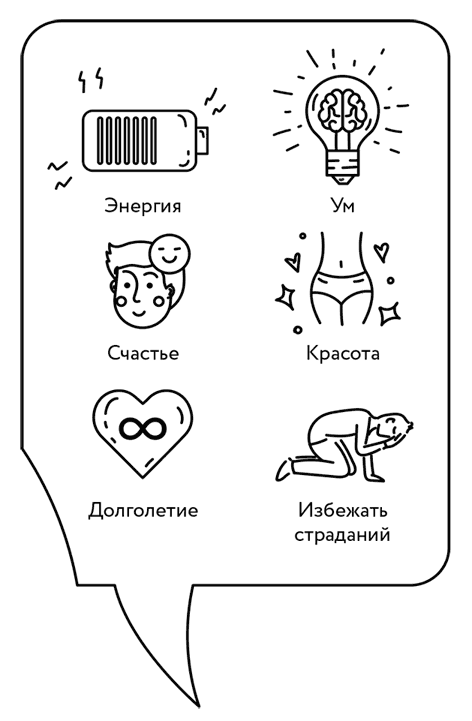
\includegraphics[width=0.4\textwidth]{willpower/pic1.png}

%   На кожным сваім навучальным курсе я пытаю: «Навошта людзі прыйшлі вучыцца здароўю?» Часьцей за ўсё я чую наступныя адказы:
  %((карцінка: Энэргія Розум Шчасьце Прыгажосьць Даўгалецьце Пазьбегнуць пакутаў))
% \end{figure}

\subsection*{Пазьбегнуць дыскамфорту, пакутаў і болю.}

Людзі зьвяртаюцца да курсу ўмацаваньня здароўя, каб вырашыць праблемы, якія ўжо існуюць. Хваробы спустошваюць нашыя рэсурсы, робяць нас больш адчувальнымі і слабымі. Умацаваньне ж здароўя ня толькі дапамагае нам прапампаваць арганізм, але і павышае ступень кантролю над сваім целам, што прыводзіць да памяншэньня болевае адчувальнасьці, паляпшэньня стану нават пры існых хваробах.

Здаровы лад жыцьця вельмі эфэктыўны для прадухіленьня захворваньняў, нават анкалёгіі. Высьветлена, што імавернасьць захворваньня на рак у~здаровага чалавека на 40\,\% ніжэйшая, чым у~чалавека са слабым здароўем. Нават калі адэпт ЗЛЖ хварэе, то рызыка сьмяротнага зыходу скарачаецца на 14--60\,\%.

\subsection*{Павысіць узровень энэргіі, разумовую і фізычную працаздольнасьць.} 
Сёньня многія прыходзяць да мяне па здароўе, але называюць яго інакш~--- энэргіяй. Такі запыт узьнікае, калі чалавек пачуваецца добра, але сутыкаецца з~падвышанай нагрузкай. Часта людзі адмаўляюцца ад пэрспэктыўнай працы ці пашырэньня бізнэсу з~прычыны стомленасьці, выгараньня. Іх звыклы ўзровень здароўя недастатковы, і каб адаптавацца да новых патрэбаў і ня выгараць, трэба павялічваць «запас здароўя». Не ахвяруйце здароўем дзеля працы, умацоўвайце здароўе і працуйце з~задавальненьнем! Упэўнены, што мацнейшае здароўе забясьпечыць вам і высокую працаздольнасьць без выгараньня.

\paragraph{Добрая навіна: такая неадаптыўнасьць не канчатковая, гэты навык трэніруецца і разьвіваецца.} Здароўе становіцца суперсілай, бо чым большы ваш адаптыўны рэсурс, тым больш вы можаце зрабіць і тым «вышэй скокнуць». Тое, што ў~слабога чалавека зь нізкім узроўнем энэргіі выкліча стому, чалавека з~высокім узроўнем энэргіі ня спыніць. Чым вы энэргічнейшы, тым лягчэй атрымліваеце тое, чаго хочаце. Многія ўжо зразумелі, што галоўная каштоўнасьць~--- гэта ня час, а~менавіта энэргія: любое адхіленьне ад оптымуму вядзе да зьніжэньня рэсурсаў здароўя і энэргічнасьці. Калі наш арганізм толькі мяркуе магчымы дэфіцыт сілаў, пагрозу свайму стану, ён на аўтапілёце пераходзіць у~«рэжым эканоміі».

\paragraph{Менавіта багацьце рэсурсаў здароўя дазваляе нам шчодра выкарыстоўваць свае сілы і накіроўваць іх у~поўным аб'ёме на важныя задачы.} Энэргія пачынаецца з~фізычнага ўзроўню, дзе яе забясьпечваюць харчаваньне, рух, сон. З фізычнага ўзроўню яна пераходзіць на псыхалягічны, дзе рэалізуецца ў~стрэсаўстойлівасьці і ўменьні канцэнтраваць увагу. Далей, на асабістым і сацыяльным узроўнях, яна раскрываецца ўжо ў~выглядзе мэтаў, каштоўнасьцяў, сэнсаў, якія і кіруюць нашымі дзеяньнямі.

\tipbox{Жаданьне стаць моцным чалавекам, нарошчваць асабістыя рэсурсы, разьвіваць здольнасьці, воля да жыцьця і да ўлады над сабой, інстынкт выжываньня й самазахаваньня~--- гэта натуральныя і здаровыя заахвочвальныя імпульсы, якія мае кожны чалавек.}

Прыслухайцеся да сябе, прыслухайцеся да свайго цела~--- яно хоча жыць напоўніцу. Дайце сабе гэтую магчымасьць~--- жыць здаровым і энэргічным кожны дзень вашага жыцьця.

\subsection*{Стаць больш прыгожым і прывабным.}

Аздараўленьне? Па-першае, гэта прыгожа. Гэта запраграмавана эвалюцыйна: прывабнасьць успрымаецца як здароўе. Пры гэтым размова ідзе ня толькі пра фізычную прывабнасьць, але і пра псыхалягічную ўстойлівасьць. Прапорцыі асобы, сымэтрыя, хада, суадносіны талія-сьцёгны, пах і іншыя «прыкметы прыгажосьці», вядома, маюць вялікае значэньне. Але здаровы чалавек таксама разьняволены, харызматычны, уважлівы да іншых і тым самым прыцягвае ўвагу.

\textbf{Псыхалягічнае здароўе і ўпэўненасьць ня менш прыкметныя, чым фізычная прыгажосьць: нават «бляск вачэй»~--- гэта ня проста мэтафара, а~дастаткова дакладны паказьнік здароўя.}

Я атрымліваю эстэтычнае задавальненьне ад здаровых людзей, побач зь імі прыемна знаходзіцца, зь імі прыемна мець справы. Заўважу, што, калі ты здаровы, наладжваюцца і адносіны з~самім сабой: нашмат больш радасна жыць, калі чалавек у~люстэрку выдатна выглядае. Вашае жаданьне быць прыгожым натуральнае, падтрымлівайце і заахвочвайце яго!

\subsection*{Жыць даўжэй.}

Страх сьмерці і нямогласьці палохае людзей. Часта здароўе ўспрымаецца як магчымасьць пражыць даўжэй, пазьбегнуць або мінімізаваць бездапаможнасьць і крохкасьць старэчых гадоў, падоўжыць ня проста гады, а~менавіта актыўны час свайго жыцьця. Бо цяпер, на тле павелічэньня працягласьці жыцьця, расьце колькасьць хваробаў, якія азмрочваюць апошнія гады самога чалавека і стан яго навакольных.

\emph{Здаровы лад жыцьця сам па сабе ня можа радыкальна падоўжыць жыцьцё, а~супердоўгажыхары ў~большасьці сваёй маюць да гэтага генэтычную схільнасьць. Але простыя правілы падтрыманьня здароўя могуць у~сярэднім падоўжыць жыцьцё мужчынаў на 7--8 гадоў, а~жанчынаў~--- на 10 гадоў, а~таксама прыкметна зьменшыць рызыку многіх захворваньняў.}

Вы ня проста пражывяце даўжэй, але яшчэ й зможаце даўжэй заставацца маладым, аддаляць час пачатку захворваньняў. Гэта ў~вашых руках. І самае важнае: здароўе вельмі моцна паляпшае якасьць жыцьця практычна ва ўсіх яго аспэктах!

\subsection*{Стаць больш шчасьлівым.}

Пытаньне шчасьця~--- гэта таксама шмат у~чым пытаньне здароўя. Бо якасьць нашага розуму~--- гэта якасьць усяго нашага жыцьця. Няўжо можа быць здаровым няшчасны чалавек? Вядома не! Парадокс: маючы нашмат больш, чым нашы продкі, мы ня проста ня сталі шчасьлівейшымі, але й наадварот~--- бо дэпрэсія становіцца ўсё больш распаўсюджанай.

Дэпрэсія можа ўзьнікаць у~сувязі з~мноствам біялягічных чыньнікаў, у~тым ліку атлусьценьне, хранічнае запаленьне, парушэньні працы шчытападобнай залозы, зьніжэньне ўзроўню тэстастэрону і да т.~п., а~ня толькі праз стрэс.

Вялікае значэньне мае і генэтыка: узровень самаадчуваньня на 35--40\,\% вызначаецца генамі. Напрыклад, носьбіты «доўгіх» варыяцый сератанінавага гену 5-HTTLPR шчасьлівейшыя за ўладальнікаў «кароткіх» варыяцый. А мо справа ў~нізкім узроўні літыю ў~пітной вадзе ці дэфіцыце фолевай кісьлі? Як бачыце, пытаньне шчасьця шмат у~чым злучанае з~нашай біялёгіяй.

\textbf{Калі вы часта і падоўгу пачуваецеся няшчасным~--- гэта можа быць сымптомам захворваньня. А для шчасьця патрэбнае як фізычнае, так і псыхічнае здароўе.}

Шчасьце~--- гэта досьвед і паўната жыцьця. Ня проста валоданьне грашыма, але й магчымасьць больш патраціць асабіста на сябе: на здароўе, на трэнэра, на псыхатэрапэўта. Шчасьце~--- гэта працэс, практыка, а~ня вынік. І яму, як і любому іншаму навыку, можна навучыцца. Імкненьне да шчасьця~--- гэта неад'емнае права кожнага чалавека.

\emph{Арыстоцель лічыў, што шчасьце~--- гэта ня так геданія, то бок задавальненьне ад ежы або музыкі, як эўдэмонія~--- задавальненьне ад правільнага жыцьця.}

Шчасьце~--- гэта ня кайф, эўфарыя, задавальненьне ці проста перавага пазітыву над нэгатывам. Навукоўцы давялі існаваньне так званага геданістычнага парадоксу~--- сьвядомае імкненьне да шчасьця або задавальненьня зьніжаюць іх. Сапраўды, спробы дасягнуць шчасьця праз самастымуляцыю ня маюць сэнсу.

\emph{Буда параўноўваў пачуцьцёвыя задавальненьні з~косткай бязь мяса, кінутай сабаку. Калі ён пачынае грызьці сухую костку, то яе вострыя краі раняць дзясны сабакі, цячэ кроў. Сабаку здаецца, што гэта сакавітая і смачная костка, і стараннасьць ягоная адно павялічваецца. Спрабуючы бегчы за задавальненьнем, мы толькі губляем шчасьце.}

Шчасьце~--- гэта сэнс, мэта, уцягнутасьць. Ужо некалькі дзесяцігодзьдзяў філёзафы гавораць пра «эпідэмію бессэнсоўнасьці», якая спараджае экзістэнцыйны вакуум. Прычыны крызісу~--- прыгнёт і аслабленьне біялягічных інстынктаў, разбурэньне традыцыйных роляў і малая колькасьць людзей, здольных самастойна ствараць сэнсы ў~сваім жыцьці. Таму многія запаўняюць унутраную пустэчу нездаровымі паводзінамі.

Шчасьце~--- гэта і радасьць ад раскрыцьця свайго патэнцыялу, і стасункі зь іншымі людзьмі. У больш шчасьлівых людзей болей блізкіх і якасных сувязяў. Нашыя сацыяльныя сувязі~--- гэта своеасаблівы буфер ад удараў жыцьця. Нізкі ўзровень сьвядомасьці і «блуканьне розуму» зьмяншае ўзровень шчасьця, а~вось практыка ўсьвядомленасьці або стан патоку павялічваюць яго.

Кожны з~рэсурсаў здароўя, якія мы будзем вывучаць у~гэтай кнізе, мае прамое дачыненьне да шчасьця, бо шчасьлівыя людзі заўважна даўжэй жывуць і меней хварэюць. Таму я спадзяюся, што кніга зробіць вас ня толькі больш здаровымі, але і больш шчасьлівымі.


\subsection*{Пытаньні і заданьні}

1. Для дасягненьня якіх мэтаў вам патрэбнае здароўе? Ці хопіць вам таго, што ёсьць у~вас цяпер? Колькі гадоў вы хацелі б пражыць?

2. Якія вашыя фізычныя і псыхічныя характарыстыкі падвысяць імавернасьць дасягненьня вашых мэтаў? Вам важна быць больш уважлiвымi, прыгожымі, разумнымi, энэргiчнымi? Што для вас значыць быць шчасьлівым?

3. Ці ведаеце вы некага, хто быў вымушаны скончыць праект, пакінуць працу з~прычыны здароўя? Ці магчыма, што нагодай была не сама праца, а~нізкі ўзровень здароўя?


\section{Парадокс здароўя}

Самая вялікая пагроза здароўю~--- гэта страта веры ў~сябе, у~сваю здольнасьць нешта зьмяніць. Здароўе больш за напалову залежыць ад нашага жаданьня і нашых сьвядомых намаганьняў. Здароўе~--- гэта стыль мысьленьня, самаідэнтыфікацыя, імкненьне да самарэалізацыі, воля да жыцьця. Страціўшы гэтую волю, мы губляем ня проста здароўе, мы губляем сябе. 

\tipbox{Усё, што мы робім сёньня,~--- гэта або інвэстыцыя ў~нашую будучыню, або крэдыт у~сябе ў~будучыні.}

Умацаваньне здароўя сёньня зробіць нас больш здаровымі заўтра, празь месяц, празь 10 гадоў. Калі ж мы ўвесь час бяром пазыку ў~свайго здароўя за кошт недасыпу, пераяданьня і злоўжываньняў, то непазьбежна прыйдзе час плаціць па рахунках~--- заўчаснай старасьцю, хваробамі й пакутай. Як па-філязофску заўважыў Сакрат, «здароўе~--- ня ўсё, але ўсё без здароўя~--- нішто».

\subsection*{Піраміда здароўя.}

Уявіце сабе нездаровага чалавека: у~яго лішняя вага, ён харчуецца абы-чым і хаатычна, мала рухаецца, шмат ляжыць, у~яго няма жаданьня і настрою вучыцца і разьвівацца, у~яго мала энэргіі, ён увесь час шукае, чым бы ўзбадзёрыцца, ён залежны ад чужой думкі, яму цяжка кантраляваць свае імпульсы. А акрамя таго, у~яго падвышаны ціск, тлустая пячонка, акнэ, бессань і шмат іншых непрыемных сымптомаў.

Уявіце, што такі чалавек атрымае ідэальнае цела. Як хутка ён зьвядзе яго да зыходнага стану? Падобна, справа ня ў~целе і ня ў~генах. А зараз возьмем іншую сытуацыю. Актыўны мэтанакіраваны здаровы чалавек атрымае такое нездаровае цела. Няўжо ён зьмірыцца з~гэтым і прыдумае апраўданьні, каб пакінуць усё, як ёсьць? Не, ён пачне мэтаскіраваную працу, выбудоўваючы сваю піраміду здароўя.

Псыхоляг Абрахам Маслоу «пабудаваў» сваю знакамітую піраміду патрэбаў, і здароўе выбудоўваецца паводле падобнай схемы:

\begin{enumerate}
  \item У аснове піраміды ляжаць \textbf{харчаваньне і рух}, бо кантраляваць сваю талерку прасьцей за ўсё, а~бяз рухальнай актыўнасьці нічога працаваць толкам ня будзе.
  \item На наступнай прыступцы пачынаем \textbf{прыбіраць вакол сябе}: вычышчаем усё сьмецьце са свайго жыцьця, як бытавое, так і інфармацыйнае. Сьпім мацней, набіраем больш сілаў і энэргіі. Зьмены фізычныя прыводзяць да таго, што наш мозг пачынае працаваць лепей.
  \item Далей прапампоўваем \textbf{усьвядомленасьць і стрэсаўстойлівасьць}, каб лепей даваць рады зьменам і больш актыўна ўкараняць новае ў~сваё жыцьцё. Дадаецца матывацыя і стрэсаўстойлівасьць, зьяўляецца жаданьне палепшыць сваё жыцьцё. Мы пачынаем складаць пляны і рэалізоўваць іх, усьвядомленасьць дапамагае нам лепш вучыцца на памылках, мяняцца і адаптавацца.
  \item Вяршыня піраміды~--- гэта сацыяльны статус, нашае асяродзьдзе, пытаньні \textbf{самаідэнтычнасьці й сэнсу жыцьця}. Вырашыўшы базавыя пытаньні са сваім здароўем, мы шукаем годнае прымяненьне сваім сілам і здольнасьцям. Сэнс надае сілы і напаўняе энэргіяй нашыя дзеяньні.
  \item Затым мы зьмяняем сваё асяродзьдзе і прыбіраем прастору вакол піраміды: \textbf{«праводзім рэвізію» нашага асяродзьдзя}, пераязджаем у~больш прыгожае і здаровае месца. Думаем пра экалёгію і паветра, імкнёмся да справядлівага і здаровага грамадства ня толькі для сябе, але й для іншых. Так выглядае піраміда здароўя, пачынаючы ад выбару прадуктаў кожны дзень і заканчваючы палітычнымі патрабаваньнямі. Мы жывыя, пакуль мяняемся, і мы можам станавіцца яшчэ больш здаровымі.
\end{enumerate}

% \begin{figure}[htb!]
%   \centering
%   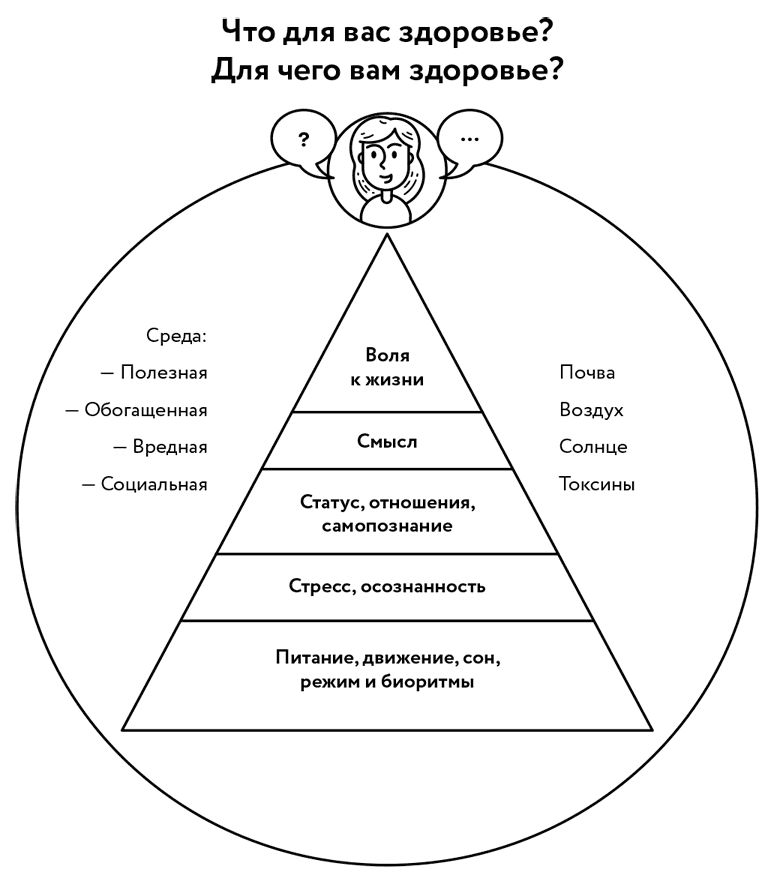
\includegraphics[width=0.8\textwidth]{willpower/pic2.png}
  %((карцінка: Што для вас здароўе? Навошта вам здароўе? / Асяродзьдзе: -карыснае -узбагачанае -шкоднае -сацыяльнае / Воля да жыцьця / Сэнс / Статус, стасункі, самаспазнаньне / Стрэс, усьвядомленсьць / Харчаваньне, рух, сон, рэжым і біярытмы / Глеба / Паветра / Сонца / Таксыны))
% \end{figure}

Мы падвышаем сваю волю да жыцьця і волю да ўлады, пераўтвараючы асяродзьдзе вакол сябе, робячы яго больш здаровым. Мы робім сьвет здаравейшым, а~здаровы сьвет яшчэ больш умацоўвае наша здароўе. Пачніце выбудоўваць сваё здароўе ад сёньня. Агледзьцеся: што вы можаце зрабіць для здароўя? Падумайце, якія вашыя дзеяньні можна зрабіць яшчэ больш здаровымі?

\subsection*{Парадокс здароўя.}

Мы жывём у~дзіўным часе: у~нас болей улады над хваробамі і самімі сабой, чым калі-кольвек у~чалавечай гісторыі, але чым у~больш здаровым грамадстве людзі жывуць, тым часьцей скардзяцца на здароўе. Гэтае назіраньне назвалі «парадоксам здароўя». Усё больш людзей знаходзяць у~сябе трывожныя сымптомы і адчуваюць большую незадаволенасьць сваім станам.

Мы жывём даўжэй, але пачынаем хварэць усё раней. Мы гонімся за камфортам, але цяпло, здаволеньне і калярыйная ежа на адлегласьці выцягнутай рукі прыводзяць да нездароўя. Эвалюцыйна ўцякаючы ад голаду, мы трапляем у~пастку пераяданьня. Працуючы ўсё больш, мы выгараем, і нам становяцца абыякавыя плады нашага посьпеху. Імкнучыся пацешыцца, адпачыць, зьняць стрэс, мы пападаем у~пастку залежнасьцяў. Вызваліўшыся ад адных хваробаў, мы сустракаем іншыя.

\subsection*{Парадокс таблеткі.}

Я часта бачу, што людзі чакаюць ад мяне чароўнай таблеткі, але ня хочуць карыстацца праверанымі эфэктыўнымі сродкамі. «Гэта вельмі проста і нудна,~--- кажуць яны,~--- а~дзе ж навука?» Прагрэс навукі спараджае ў~шматлікіх людзей чаканьне, што нейкія прэпараты ці апараты змогуць чароўнай чынам іх аздаравіць. Аднак дасюль ня вынайдзеная і наўрад ці зьявіцца ў~найбліжэйшай будучыні таблетка, якая зробіць вас стрэсаўстойлівымі і ўсьвядомленымі, худымі і мускулістымі. Таму імкніцеся ня піць таблеткі, каб быць здаровымі, а~быць здаровымі, каб ня піць таблеткі.

\paragraph{Абсалютная большасьць дадаткаў не дае прыкметнага эфэкту здаровым людзям.} А вось здаровы лад жыцьця~--- працуе, робіць нас лепшымі і мацнейшымі. Менавіта сьвядомыя ўважлівыя дзеяньні стымулююць разьвіцьцё, а~не пасіўнае спажываньне «аздараўленчых» прадуктаў. Многія людзі даюць нырца ў~ЗЛЖ, але атрымліваюць толькі праблемы са здароўем. Рыба на абед больш эфэктыўная, чым Амега-3 у~капсулах; прыём вітаміну D не заменіць часу, праведзенага на сонцы; міястымулятары не разьвіваюць цягліцы, а~рэгулярныя практыкаваньні працуюць на 100\,\%.

На жаль, лекары і мэдычнае асяродзьдзе не пасьпяваюць за ўсплёскам масавага попыту на здаровы лад жыцьця і практычна не даюць пэўных навуковых адказаў на пытаньні менавіта прафіляктыкі, умацаваньня здароўя, больш факусуючыся на лячэньні ўжо існых захворваньняў. Гэта прывяло да зьяўленьня вялікай колькасьці інста-дактароў, аматараў і шарлятанаў.

\subsection*{Парадокс «аздараўленьня».} 

Я не лічу посьпехам, калі мой кліент схуднеў. Посьпех~--- гэта стабільнае падтрыманьне здаровай вагі і аптымальнага харчаваньня на працягу доўгага часу. Многія лічаць, што здароўе~--- гэта нейкі аднаразовы акт. Напрыклад, можна цэлы дзень ляжаць на канапе, а~ўдарная трэніроўка ўсё кампэнсуе. Або можна есьці абы-што~--- і аздаравіцца за тыдзень разгрузачнага галаданьня. Можна паводзіць сябе подла і агідна, а~затым памэдытаваць ці пакаяцца. Можна жыць сярод бруднага паветра, але выяжджаць раз на тыдзень у~лес. На жаль, гэта так не працуе, і кампэнсаваць шкоду свайму арганізму эпізадычнымі дзеямі не атрымаецца. Ня «чысьціце» цела і розум ад бруду, а~трымайце цела і розум у~чысьціні.

Здароўе~--- гэта і ёсьць само жыцьцё, здароўе~--- гэта тое, што мы робім кожны дзень, гэта звычкі, гэта тканка нашай штодзённасьці. Таму так важна фармаваць здаровы лад жыцьця, здаровыя звычкі. Акрамя таго, здароўе, як і гонар, трэба берагчы замалада. Зрэшты, пачаць ніколі ня позна і, зьмяніўшы свой лад жыцьця ў~любы момант, можна атрымаць пэўную карысьць. Я спадзяюся, што гэтая кніга дапаможа вам скласьці сваю сыстэму здароўя і ўкараніць яе ў~паўсядзённае жыцьцё.

\subsection*{«Мэдыцына для ўсіх» і «мэдыцына для кожнага».}

Прагрэсіўнай формай мэдыцыны зьяўляецца доказная мэдыцына, якая вывучае тое, што працуе на вялікіх выбарках людзей, усярэдніваючы значэньні. Гэта добра для лекараў, у~якіх ёсьць 15 хвілінаў на пацыента. Але тое, што добра для людзей «у сярэднім», неабавязкова выявіцца карысным асабіста для вас.

Арганізм кожнага чалавека мае свае асаблівасьці і нюансы, таму як мэдычныя прэпараты, так і мэтады аздараўленьня працуюць для ўсіх па-рознаму. Для адных гэты прэпарат будзе карысны, іншыя атрымаюць адно пабочныя эфэкты. У адных рэжым трэніровак прывядзе да інтэнсіўнага цяглічнага росту, у~іншых~--- амаль да нулявых вынікаў. Жывёльныя насычаныя тлушчы шкодзяць людзям з~пэўнымі генамі, у~той час як астатнія могуць есьці іх бяз шкоды для здароўя.

Таму мэдыцына імкнецца стаць пэрсаналізаванай, разьбіваючы людзей на розныя групы і падбіраючы для кожнага тыпу аптымальныя лекі. У аздараўленьні важна ня проста прытрымлівацца агульных парадаў, а~шукаць тую, што лепей за ўсё спрацуе менавіта для вас. Вывучыце сябе, каб дзейнічаць эфэктыўна! \textbf{Для гэтага трэба валодаць вялікай колькасьцю інфармацыі аб сваім здароўі і адсочваць вынікі сваіх дзеяньняў.} Толькі так мы можам разумець, ці ў~слушным кірунку рухаемся.

Існуе меркаваньне, што здароўе~--- гэта вельмі затратна, і дазволіць яго сабе могуць ня ўсе. Я зьбіраюся давесьці, што гэта ня так. Здароўе~--- гэта інвэстыцыі, а~ня траты. Рэарганізуючы свой лад жыцьця, вы будзеце атрымліваць такі прыбытак, як задавальненьне, вызвалены час і зэканомленыя выдаткі.

\paragraph{Здароўе дае жыцьцё, час і энэргію, а~энэргічнасьць дае вам больш здароўя.} Сучасная навука і мэдыцына даюць нам мноства магчымасьцяў папярэдзіць і запаволіць разьвіцьцё шматлікіх хваробаў. Для таго каб стаць яшчэ здаравейшым любому здароваму чалавеку, а~хвораму~--- умацаваць сваё здароўе, не патрэбныя дарагія прэпараты або адмысловыя прыборы~--- усё неабходнае ўжо ёсьць у~вашых руках. 

\textbf{Любы чалавек, любога ўзросту, зь любымі магчымасьцямі, у~любы час можа пачаць дзейнічаць і станавіцца здаравейшым і мацнейшым.}

\subsection*{Навошта мне чытаць пра здароўе, калі ў мяне нічога не баліць?}

Многія людзі ўспрымаюць здароўе і аздараўленьне як нешта, што датычыцца толькі зьмяншэньня рызыкі захворваньняў. Але гэта ня так: аздараўленьне~--- гэта ня толькі зьніжэньне рызыкі, гэта неад'емны кампанэнт асабістага разьвіцьця. Гэта паляпшэньне працы нашага розуму, разьвіцьцё нашай асобы, павышэньне кагнітыўных здольнасьцяў, павелічэньне рэсурсаў, сілаў, грошай, часу, уплыву.

\paragraph{Здароўе~--- гэта самаразьвіцьцё, бясконцы працэс супрацьстаяньня разбуральнаму дзеяньню часу.} Пакуль навука ня можа прапанаваць нічога прарыўнога ў~лекаваньні галоўнага ворага~--- старэньня. Выкарыстоўваючы ўсе сучасныя веды, мы можам падоўжыць сабе жыцьцё да 90+, зрабіўшы гэтыя доўгія гады~--- здаровымі. Для большага выніку добра было б выйграць у~генэтычнай лятарэі, але адваротная сытуацыя ня значыць, што трэба здавацца. Кожны год усё больш вучоных далучаюцца да барацьбы за нашае здароўе, зьяўляецца ўсё больш новых мэтадаў лекаваньня. Мы бачым прыкметны прагрэс у~шматлікіх галінах мэдыцыны: павышэньне эфэктыўнасьці лячэньня розных відаў раку, хваробаў сэрца, мозгу. Умацоўваючы здароўе і падаўжаючы жыцьцё, мы можам дачакацца моманту, калі тыя праблемы са здароўем, што сёньня ўяўляюцца невырашальнымі, могуць быць лёгка вырашаныя заўтра.

А пакуль здаровы лад жыцьця дапаможа зрабіць старэньне аптымальным. Бо і старэць можна высакародна, пакрываючыся пацінай, як срэбра, а~не рассыпаючыся ў~іржавую пацяруху, як бляха. Не скісаючы, як таннае віно, а~набываючы глыбокія адценьні смаку, як дарагія віны з~«патэнцыялам старэньня». 

\emph{Старэючы, вы хочаце скіснуць або стаць высакародным віном? Вы аддаяце перавагу знасіцца ад працы ці заржавець ад бязьдзейнасьці?}

\subsection*{Пытаньні і заданьні}

1. Наколькі здаровае тое, што ёсьць у~вашым жыцьці: ежа, рух, камунікацыя, праца, сям'я, асяродзьдзе, сябры, мэты, адпачынак? Ацэніце кожную сфэру па дзесяцібальнай шкале.

2. Хто зь людзей, якіх вы ведаеце, радыкальна зьмяніў сваё жыцьцё, пачаўшы паляпшаць здароўе? Што для іх спрацавала? Хто з~вашых герояў ці ролевых мадэляў надае адмысловую ўвагу здароўю? А хто спрабаваў «змахляваць», зьвяртаючыся да сумнеўных спосабаў «аздараўленьня»?

3. Якім вы сябе бачыце ў~старасьці? Здаровым бадзёрым пэнсіянэрам, які вандруе па сьвеце зь невычэрпнай цікаўнасьцю, ці тым, хто мадзее старцам з~мноствам хваробаў?


\section{Здароўе як вайна з~сабой і сьветам}

Многія людзі прыходзяць да мяне на кансультацыю з~такім настроем, быццам яны сабраліся на вайну са сваім арганізмам. І мне прыемна бачыць, што падчас нашай гутаркі ў~іх прачынаецца цікавасьць, а~напруга сыходзіць,~--- бітвы звычайна не пакідаюць такога посмаку. Я вельмі рады, калі чалавек адчувае цікавасьць да свайго арганізму і гатовы шукаць, як здаволіць свае патрэбы здаровымі спосабамі, а~не ґвалтаваць сябе строгімі дыетамі і зьнясільвальнымі трэніроўкамі.

Клясычная мэдыцына фармавалася ў~тыя гады, калі асноўныя пагрозы для здароўя былі вонкавымі: таксыны, інфэкцыі, голад, пашкоджаньні. Зь імі трэба было змагацца, іх трэба было зьнішчаць. Такі падыход прывёў да ўзьнікненьня мэдыцынскай мэтафары «вайны», бітвы за здароўе. Але за апошнюю сотню гадоў усё зьмянілася, і на сёньня галоўныя прычыны хваробаў і сьмерцяў~--- унутраныя, так званыя «хваробы цывілізацыі»: сардэчна-сасудзістыя захворваньні, пухліны, дыябэт, атлусьценьне, дэпрэсія. \textbf{І што атрымліваецца~--- цяпер нам трэба ваяваць са сваім целам, розумам, псыхікай?!}

\emph{«У вас хвароба Х.~--- Як непрыемна.~--- Яна лечыцца здаровым харчаваньнем і фізычнай актыўнасьцю.~--- Жахліва, о не, толькі ня гэта!»} Калі мы кажам пра здаровы лад жыцьця, то для шматлікіх людзей гэта выглядае як неабходнасьць прымусу сябе да таго, чаго ня хочацца, адмовы ад таго, што падабаецца, і наогул пастаяннымі абмежаваньнямі. Мэдыя, на жаль, таксама рэдка трансьлююць ідэі балянсу або самавывучэньня, заяўляючы: «забі ў~сабе слабасьць», «зьнішчы і выкіні цукар», «зьеж гэта празь сілу», «трэніруйся да крывавага поту» і да т.~п.

Сьвет успрымаецца як агрэсіўнае месца, дзе нам увесь час пагражаюць хваробатворныя бактэрыі, дзе спакушаюць прадаўцы марозіва, дзе крадуць нашу ўвагу і нават душу смартфоны, у~лёгкія імкнецца патрапіць бруднае паветра, а~ў мозг увесь час залятаюць дрэнныя навіны. \textbf{Атрымліваецца, што нам трэба быць пастаянна пільнымі, каб не прапусьціць пагрозу, рэгулярна «чысьціць» сваё цела ад таксынаў і стымуляваць «абарону» арганізму.}

\subsection*{Канцэпцыя «крэпасьці ў~аблозе».} 

Праз такі «парадак дня» наш мозг разглядае наша існаваньне асобна ад асяродзьдзя, заўважае ўвесьчасныя напады шкодных чыньнікаў і зводзіць сваё разьвіцьцё адно да спосабаў распрацоўкі больш дасканалага ўзбраеньня. Роля самога чалавека (жаўнера) нязначная, бо камандуюць і прымаюць рашэньні толькі палявыя камандыры (урачы), а~мы пачуваемся адстароненымі як ад прыняцьця рашэньняў, так і ад разуменьня таго, што насамрэч адбываецца. 

\emph{Ёсьць жарт пра тое, што «магчымасьці мэдыцыны бязьмежныя, абмежаваныя толькі магчымасьці канкрэтнага пацыента''. Успомніце, як непрыемна, калі лекары абмяркоўваюць ваш стан, цалкам ігнаруючы вас і вашыя пытаньні!}

Такая ваенная мэтафара добра пасуе да лекаваньня канкрэтнай хваробы. Аднак далёка не заўсёды мэты і сродкі «лекаваньня хваробаў» супадаюць з~«умацаваньнем здароўя». Калі мы паглядзім на здароўе як на балянс арганізму і навакольнага асяродзьдзя, балянс цела і розуму, то зможам зразумець, што зьяўляемся часткай асяродзьдзя: мы адаптуемся да яго ды імкнёмся да раўнавагі.

Барацьба са шкоднымі звычкамі таксама ўспрымаецца як працяглая бітва, дзе частыя паразы і вялікія ваенныя выдаткі. Разуменьне дзейных мэханізмаў шкодных звычак дапамагае нам убачыць, якія з~нашых патрэбаў яны задавальняюць, чаму яны сталі часткай нашай самаідэнтыфікацыі і як магчыма гэтыя ж патрэбы здаволіць здаровым спосабам.

\textbf{Парушэньні здароўя ўзьнікаюць у~выніку парушэньняў адаптацыі, і гэтыя зьмены далёка не заўсёды паталягічныя па сваёй ісьце, у~іх закладзены важны прыстасоўвальны мэханізм, які й дапаможа аднавіць здароўе,~--- вядома, калі правільна ім скарыстацца.} 

Сапраўдная сувязь з~самім сабой пачынаецца са шчырай цікавасьці да сябе. Таму так важна ведаць стан свайго цела і розуму, заўважаць, якія сыгналы мы даём арганізму праз наш лад жыцьця (рэжым, ежа, рух, стрэс) і як ён адказвае на гэтыя сыгналы. Разьвіцьцё такой уважлівасьці дазваляе знайсьці для сябе аптымальныя ўмовы. Бо нас хвалюе ня толькі зьніжэньне рызыкі захворваньняў у~будучыні, але й наш стан сёньня: узровень энэргіі, смак жыцьця, камфорт знаходжаньня ў~целе, лёгкасьць і задавальненьне ад кожнай пражытай гадзіны.

Умацаваньне здароўя~--- гэта сума нашых паўсядзённых рашэньняў і ўчынкаў, якія мы робім зь любоўю і задавальненьнем, а~не баявыя задачы накшталт схуднець да лета, напампаваць цягліцы за месяц, хутка вырашыць праблему са сном, ачысьціць арганізм за дзень, прыбраць стрэс за вечар, адаспацца на тыдзень, прапіць вітаміны, ня есьці цукар, пакутуючы на цукровую залежнасьць, і ўсё гэта без разуменьня свайго стану і зыходных дадзеных. Калі мы думаем пра здароўе як пра балянс, то нам трэба ўмець ацэньваць, з~аднаго боку, свой рэсурс, з~другога~--- свой лад жыцьця. Бяз гэтага балянс і ўкараненьне пэрсаналізаваных зьменаў на доўгатэрміновай аснове будуць немагчымыя.

\emph{Упэўнены, што вы зможаце зьмяніць сваё здароўе на доўгатэрміновай аснове, а~не здавольвацца адно спробамі зьмяніцца. Бо, як казаў Буда, «ваду праводзяць арашальнікі, паляўнічыя апэрваюць стрэлы, цесьляры працуюць з~дрэвам, а~мудрыя людзі~--- над сабой».}

\subsection*{Пытаньні і заданьні}

1. Прааналізуйце мэтафары, якія вы выкарыстоўваеце для апісаньня свайго цела. Замяніце іх на канструктыўныя і спагадлівыя. Хай гэта будзе не «гультайскі трыбух», а~«мудры арганізм, навойстраны мільёнамі гадоў эвалюцыі».

2. Ці часта вы прымушаеце сябе рабіць нешта толькі таму, што гэта «карысна»? Як вы пры гэтым пачуваецеся?

3. Як вы ставіцеся да навакольнага асяродзьдзя? Гэта для вас цудоўнае месца, дзе багата карыснага для здароўя, ці вы бачыце толькі бруднае паветра, атручаныя акіяны і забруджаныя пэстыцыдамі землі? Зірніце на навакольны сьвет як на крыніцу здароўя без «ваенных» кагнітыўных фільтраў.


\section{Гісторыя здароўя}

Мы заўсёды імкнуліся зразумець, чаму ўзьнікаюць праблемы ў~арганізьме і што трэба рабіць для таго, каб захаваць здароўе. Пазыцыя людзей таксама прайшла шлях ад «чалавека пасыўнага» перад абліччам пагрозаў да «чалавека актыўнага», які кіруе сваім здароўем.

\subsection*{Здароўе як сьвятасьць і чысьціня.}

Здавён-даўна людзі спрабавалі «выгнаць» хваробу зь цела рознымі спосабамі: існавалі практыкі выгнаньня духаў ці дэманаў, замольваньня грахоў і «нячыстых» учынкаў. Хвароба ўспрымалася як злы дух ці пакараньне ад боства за парушэньне нейкіх правілаў. Такое ўспрыманьне хваробы мае глыбокія эвалюцыйныя карані.

Для раньніх сысуноў важную ролю ў~выжываньні граў нюх: яны вучыліся шукаць і ацэньваць ежу па паху. Калі нешта пахла дрэнна, значыць, гэтага трэба пазьбягаць. Добрыя пахі сталі выклікаць пазытыўныя эмоцыі, а~кепскія, брудныя, небясьпечныя~--- нэгатыўныя. Так склалася, што нашы вышэйшыя нэрвовыя цэнтры сфармаваліся на месцы старажытных цэнтраў, якія адказваюць за нюх.

У вышэйшых прыматаў, у~тым ліку чалавека, нюх ужо ня грае настолькі важнай ролі. Але мозг усё роўна ўспрымае навакольны сьвет праз прызму пахаў. Распазнаючы пахі, мы вызначаем «добрае» і «дрэннае». Мы часта гаворым і ацэньваем рэчы і людзей, як быццам хочам іх зьесьці.

\emph{Прыслухайцеся да сябе, калі гаворыце пра нешта «дрэннае»: брудны, неахайны, ванітоўны і гэтак далей. Гэта выклікае непрыманьне, жаданьне пазьбягаць. А вось пра «добрых» людзей ці рэчы ідзе зусім іншая размова: чысты, сьвежы, сакавіты, смачны. І гэта выклікае ў~нас жаданьне валодаць.} 

Эмацыйная ацэнка «чысты~--- брудны» закладзеная і ў~нашым самаадчуваньні. Гэта называюць «псыхалягічным забруджваньнем», калі мы адчуваем сябе бруднымі, нячыстымі, сьмярдзючымі.

\tipbox{«Псыхалягічнае забруджваньне» можа быць наступствам траўмы, стрэсу, сымптомам дэпрэсіі, зьніжанай самаацэнкі, а~таксама ўзьнікаць як наступства крытыкі, зьнявагі і здрады.}

Крыніцай падобнага адчуваньня зьяўляюцца нашыя ўласныя дзеяньні ці ўчынкі іншых людзей, а~ня нейкае «рэальнае» забруджваньне. Вы можаце пачувацца запэцканым нават пры павярхоўным кантакце зь непрыемным вам чалавекам. І ў~вас узьнікне жаданьне памыць рукі, вымыцца, каб аблегчыць пачуцьцё віны або непрыманьня. Дарэчы, ці лягчэе вам пасьля душу?

\emph{Тыповы ў~гэтым выпадку прыклад рымскага пракуратара Понція Пілата, які падчас суду над Хрыстом зьдзейсьніў прынятае сярод юдэяў рытуальнае абмываньне рук у~знак недатычнасьці да зьдзяйсьняльнага забойства. З ачышчэньнем іншага роду зьвязанае разьвіцьцё драмы ў~Старажытнай Грэцыі: танцы, музыка і сьпевы служылі лекавымі сродкамі для душы, дапамагалі дасягнуць катарсісу, г.~зн. ачышчэньня ад трывогі, зьбянтэжанасьці, неўтаймаваных жарсьцяў для вяртаньня самакантролю.}

Адчуваньне «бруду» эмацыйна непрыемнае, і, вядома, яго хочацца пазбыцца. Рэлігіі і духоўныя практыкі выкарыстоўвалі сымболіку «ачышчэньня» ў~сваіх рытуалах. Пусканьне «гнілой» ці «лішняй» крыві было папулярным мэтадам і каштавала жыцьця велізарнай колькасьці людзей, ня меншая колькасьць хваробаў лячыліся прамываньнем кішачніка. Цяпер канцэпцыя зьмянілася, і людзі змываюць ужо не грахі, а~шлакі, і разьдзіраюць іх не нячысьцікі, а~іншаплянэтнікі ці паразіты.

Рознага кшталту «дэтоксы» прапануюць пачысьціць кішачнік, печань, кроў і да т.~п. Зразумела, арганізм здаровага чалавека сам выдатна дае рады з~вывядзеньнем прадуктаў абмену, а~для рэальных інтаксікацый ці пры захворваньнях нырак існуюць адмысловыя спосабы лячэньня. \textbf{Мы ўспрымаем здароўе як чысьціню, а~фізычная яна ці эмацыйная~--- неістотна.}

\subsection*{Здароўе як балянс.} 

Старажытнагрэцкі філёзаф і лекар Алкмэон Кратонскі лічыў, што «здароўе~--- гэта гармонія процілегла скіраваных сілаў». Ідэя здароўя як раўнавагі стыхіяў у~арганізьме папулярная і на Захадзе, і на Ўсходзе: балянс «пяці стыхіяў», «інь і ян», «вадкасьцей», «дошаў», «першаэлемэнтаў», «сокаў»~--- у~розных культурах гэтыя ўяўленьні былі падобныя. Кожная школа па-свойму ацэньвала і прапаноўвала выпраўляць дысбалянсы.

Ужо згаданае кровапусканьне, напрыклад, выкарыстоўвалася і для вываду лішку «агню» зь цела, калі пры гарачках пускалі кроў для «ахаладжэньня». Гэтая працэдура прыкметна памяншала шанцы выжыць. 

\tipbox{Асабісты доктар прэзыдэнта ЗША Джорджа Вашынгтона прапісваў кровапусканьне бадай пры ўсіх яго захворваньнях: спроба вылечыць такім чынам пнэўманію, магчыма, і прывяла палітыка да сьмерці.} 

Зрэшты, донарства для многіх людзей сапраўды карыснае, а~калі ў~чалавека ёсьць лішак жалеза ў~арганізьме~--- тады й неабходнае. У пазьнейшы час ідэя балянсу адрадзілася ў~разуменьні здароўя як «згоды душы і цела», раўнавагі паміж чалавекам і тым асяродзьдзем, дзе ён жыве.

\subsection*{Здароўе як выратаваньне.} 

У шэрагу філязофскіх і рэлігійных вучэньняў сьцьвярджалася, што большасьць пакут у~жыцьці чалавека паходзяць ад невуцтва і няўменьня даць рады жыцьцёвым выклікам. Цялеснае і псыхічнае здароўе ўспрымалася як вытворнае ад разумовых намаганьняў і лічылася наступствам самаразьвіцьця.

З пункту гледжаньня стоікаў, ключ да ўсяго~--- спазнаньне «лёгасу», пошук прычынаў, а~зло~--- гэта вынік невуцтва. Практыка стаіцызму меркавала самадысцыпліну і жыцьцё паводле натуральных законаў прыроды. «Жыць у~згодзе з~прыродай» важна ня толькі ў~захаваньні фізычных законаў, але і законаў мысьленьня.

У будызьме жыцьцёвыя выпрабаваньні і жаданьні прыводзяць да пакутаў, а~хвароба~--- адзін зь відаў зямных пакутаў, якіх немагчыма цалкам пазьбегнуць. Свабода ад жарсьцяў, умеранасьць і самадысцыпліна дапамагаюць зьмякчыць пакуты.

\textbf{Важны момант: разумовая дысцыпліна магчымая ў~будызьме толькі пры выкананьні досыць строгіх правілаў ладу жыцьця, такіх як дыета, умеранасьць, мэдытацыя, мінімалізм, чалавекалюбства, спачуваньне, пазьбяганьне залежнасьцяў і да т.~п.} 

З пункту гледжаньня будыста, добра, што вы пазбавіліся ад хваробы, але было б цудоўна, калі б і астатнія людзі таксама навучыліся пазбаўляцца ад пакутаў і хваробаў.

\subsection*{Пытаньні і заданьні}

1. Каб пачувацца лепей, часьцяком досыць толькі прыбраць з~хаты, тэлефона і галовы ўсё сьмецьце, усё пачысьціць, вымыцца самому і апрануцца ў~чыстае і прыгожае. Гігіена~--- разумовая, сацыяльная, фізычная~--- гэта аснова здароўя, і няхай ваш рэфлекс ачышчэньня паклапоціцца пра вас.

2. Што выводзіць вас з~раўнавагі? Якія свае рысы ці жарсьці вы лічыце незбалянсаванымі? Чым іх можна ўраўнаважыць?

3. Ці згодныя вы з~тым, што «невуцтва~--- корань усіх пакутаў»? Ці дастаткова вы ведаеце пра свой розум і сваё цела?


\section[Антычная канцэпцыя асабістага здароўя, альбо «Як сесьці на дыету»][Антычная канцэпцыя асабістага здароўя]{Антычная канцэпцыя асабістага здароўя, альбо «Як сесьці на дыету»}


У маёй кніжнай шафе ганаровае мейсца займаюць кнігі некалькіх антычных аўтараў. Іх ідэі актуальныя і сёньня, жарты па-ранейшаму сьмешныя, а~праблемы прымушаюць задумацца. Эпоха антычнасьці стала ўзорам для ўсіх наступных часоў, сфармаваўшы ідэал чалавека~--- прыгожага душой і целам, грамадзяніна і ваяра, які нясе адказнасьць перад сабой і людзьмі. 

\tipbox{Здароўе для грэкаў было ня ўтомным «абавязкам», а~неад'емнай часткай самаразьвіцьця і самаспазнаньня. Так, нароўні з~росквітам мастацтва і зараджэньнем навукі і філязофіі, узьнікла новае разуменьне асабістага здароўя.}

\subsection*{Натуральнасьць здароўя.} 

Натуральнасьць здароўя~--- гэта датрыманьне сваёй прыроды і прыроды рэчаў. Невыпадкова на франтоне старажытнагрэцкага храма Апалёна ў~Дэльфах быў надпіс: «Спазнай самога сябе». Натуральнасьць уключала гармонію і суразьмернасьць цела і духу, раўнавагу дзейных у~арганізьме сілаў, а~яшчэ~--- гарманічныя стасункі з~асяродзьдзем. Важным лічылася прытрымлівацца сваёй прыроды і быць у~ладзе з~усім, што цябе атачае.

% \begin{figure}[htb!]
%   \centering
%   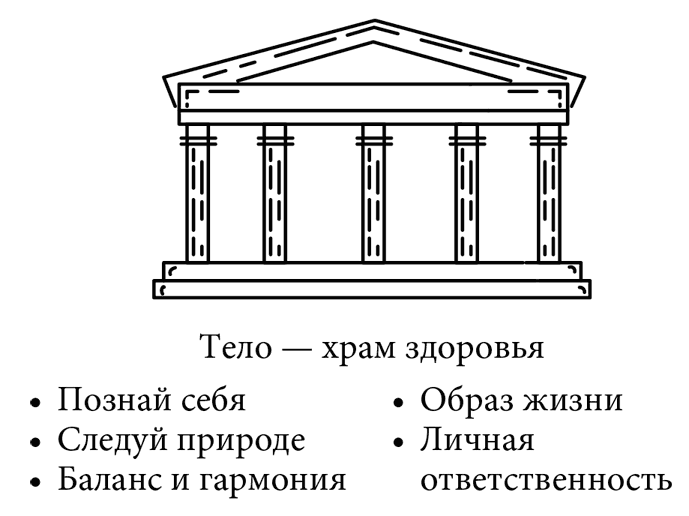
\includegraphics[width=0.6\textwidth]{willpower/pic3.png}
  %((карцінка: Цела~--- храм здароўя /~--- Спазнай сябе /~--- Трымайся прыроды /~--- Балянс і гармонія /~--- Лад жыцьця /~--- Асабістая адказнасьць))  
% \end{figure}

\subsection*{Разумнасьць здароўя.} 

Розум~--- гэта ключавы аспэкт дасягненьня здароўя: дзеля яго падтрыманьня чалавек мусіць прымаць разумныя рашэньні, быць разважлівым і апанаваць свае жарсьці. Важным кампанэнтам лічылася тое, што сёньня мы завём стрэсаўстойлівасьцю~--- «цьвёрда трываць страты і злыбеды»,~--- і аўтаноміяй~--- «не залежаць ад фартуны і вонкавых уплываў». Стоікі сьцьвярджалі, што нават пры неспрыяльных абставінах чалавек можа быць здаровым, бо ён вольны выбіраць свой лад жыцьця. Для гэтага трэба ўзгадніць свае рашэньні са сваімі асаблівасьцямі й перавагамі і жыць у~згодзе з~прыродай, выкарыстоўваючы здаровы глузд.

\subsection*{Прыняцьце сябе.} 

Зварот да самога сябе ёсьць умовай здаровага і паўнавартаснага існаваньня. Сілы для самаўдасканаленьня трэба шукаць унутры, для чаго неабходная павага да сябе, адэкватная самаацэнка. Уменьне бачыць уласныя вартасьці і недахопы~--- важная прыкмета здароўя.

\subsection*{Гармонія са сьветам.}

Унутраны лад здаровага чалавека аналягічны дасканаламу ладу сьветабудовы і ўяўляе сабой увасабленьне «Усеагульнага Вышэйшага Парадку». Здаровы чалавек не павінен выступаць супраць уласнай прыроды, а~паколькі гэтая прырода аналягічная прыродзе сьветабудовы, то здаровы чалавек не павінен мець непрымірымых канфрантацыйных адносінаў са сьветам.

\subsection*{Асабістая адказнасьць за здароўе.} 

Філёзаф Дэмакрыт заўважыў, што \emph{«здароўя просяць у~багоў у~сваіх малітвах людзі, а~таго ня ведаюць, што яны самі маюць у~сваім распараджэньні сродкі да гэтага».} Менавіта ў~антычнасьці сфармавалася ідэя асабістай адказнасьці за сваё здароўе. Для дасягненьня гэтага патрабаваліся праца, трэніроўка цела і розуму. Толькі тады можна было казаць пра па-сапраўднаму здаровага чалавека.

\subsection*{Дыета па-старажытнагрэцку.} 

Слова «дыета» за апошнія гады займела крыху нэгатыўную афарбоўку, зьвязаную з~харчовымі парушэньнямі, відавочна ненавуковымі і шкоднымі трэндамі і шматлікімі загалоўкамі ў~СМІ. Таму часта мы ўспрымаем панятак «дыета» як нешта кароткачасовае і нездаровае, характэрнае для людзей з~кампульсіўнымі паводзінамі. Але на працягу амаль трох тысячаў гадоў дыета (δίαιτα~--- \emph{грэч.}) азначала «ўклад, лад жыцьця, побыт», маючы на ўвазе лад жыцьця хворага, што вядзе да яго акрыяньня. 

\textbf{Старажытнагрэцкая навука аб тым, як зьмяняць лад жыцьця, называлася «дыетыка». Адсюль і пайшла сучасная дыета.}

Лекары-філёзафы грэчаскіх полісаў лічылі, што іх вонкавы выгляд мусіць увасабляць іх каштоўнасьці. Таму яны сачылі за харчаваньнем, займаліся спортам і практыкавалі ўмеранасьць. 

\emph{Атлет Ік Тарэнцкі атрымаў Алімпійскі вянок у~пяцібор'і ў~444 г. да н.~э., а~пасьля перамогі праславіўся як найлепшы інструктар па атлетыцы і «бацька спартыўнай дыеталёгіі». Пры падрыхтоўцы да спаборніцтваў ён практыкаваў палавое ўстрыманьне і строгую ўмеранасьць у~ядзе: панятак «абед Ікаса», як відаць, азначаў проста пустую талерку.}

У гэты пэрыяд часу, на тле культу спорту і здаровага цела, людзям з~залішняй вагой даводзілася цяжка. Да прыкладу, кіраўнік Гераклеі Дыяніс (IV стагодзьдзе да н.э.) так саромеўся сваёй паўнаты, што прымаў навакольных, седзячы ў~бочцы (ня блытаць з~Дыягенам!), зь якой тырчала толькі яго галава. У Спарце поўных людзей не было ад слова «зусім»: мужчынаў з~залішняй вагой там лупцавалі, а~потым выганялі з~горада. Есьці на самоце і ня ведаць меры ў~ядзе было складана з~прычыны правіла грамадзкіх трапэзаў (сысытыяў), дзе за абедам зьбіраліся цэлымі таварыствамі.

Пазьней слова diaeta (дыета на латыні) пачало разумецца ў~шырэйшым сэнсе~--- як умеранасьць ва ўсім. Пра гэта гаворыцца, напрыклад, у~сярэднявечным трактаце «Салернскі кодэкс здароўя» (XIV ст.): \emph{«Найвышэйшы закон мэдыцыны~--- дыету выконваць няўхільна. Будзе лячэньне дрэнным, калі забудзесься, лечачы, пра дыету. Колькі, калі, чаму, як часта і што прыдатна~--- усё гэта павінен наказваць лекар, прызначаючы дыету».}

\subsection*{Пытаньні і заданьні}

1. Ці добра вы сябе ведаеце? Апытайце пяць розных сяброў, папрасіце іх даць вам характарыстыку. Ці супадае яна з~вашымі асабістымі адчуваньнямі?

2. Хто адказвае за ваша здароўе? Хто вінаваты ў~вашых праблемах са здароўем: кепскія гены, дрэнны ўрад, нядбайныя бацькі, сапсаваная экалёгія? Вы пасіўна прымаеце ўсё як ёсьць або робіце сьвядомы выбар адносна свайго здароўя?

3. Ці прымаеце вы свае недахопы? Адмаўляючы свае асаблівасьці, мы ігнаруем і магчымасьці для зьмены. Прыміце сябе, іншага «Я» ў~вас няма. Як вашыя недахопы можна ператварыць у~перавагі?


\section{Здароўе ці хвароба, норма ці здароўе?}

Прагрэс анатоміі і фізыялёгіі пачаўся ў~эпоху Адраджэньня, і з~таго часу многія дасьледчыкі пачалі ўспрымаць цела як своеасаблівы мэханізм. Сэрца~--- помпа, сасуды~--- трубы, суставы і сухажыллі~--- блёкі і шасьцярэнькі. Здароўе мяркуе правільную працу гэтага мэханізму, іншымі словамі, здароўе~--- гэта адсутнасьць парушэньняў, хваробаў. Тады і лячэньне азначае «хутка выправіць паломку», каб чалавек мог працягнуць свой звыклы лад жыцьця.

\emph{Атэрасклератычная бляшка закрывае артэрыю? Трэба проста паставіць стэнт, які пашырае прасьвет, і хвароба вылекаваная. На жаль, у~рэальнасьці ўсё нашмат складаней.}

Шмат у~чым падыход «або здаровы, або хворы» застаецца і сёньня, калі мноства перадхваробаў або станаў, якія не адпавядаюць крытэрам хваробы, ігнаруюцца, а~скаргі людзей~--- абясцэньваюцца. \textbf{Па сутнасьці, прапануецца зьвяртацца па дапамогу толькі тады, калі разаўецца захворваньне, а~да гэтага чалавек фармальна прызнаецца здаровым.}

\emph{Было ў~вас так: адчуваеце сябе дрэнна, прыходзіце да лекара, здаяце аналізы, яны «ў норме», і выразны позірк лекара ясна дае зразумець, што шпіталь~--- гэта не месца для сымулянтаў.}

\emph{Але ж вы сапраўды пачуваецеся нездаровым!?}

Існуе такая мадэль здароўя~--- біястатычная, у~ёй здароўе разглядаецца як дыяпазон шэрагу паказьнікаў, у~якім адбываецца нармальная праца арганізма, а~хвароба~--- гэта выхад за межы нормы. Паводле гэтай сыстэмы, нормы ўніверсальныя і могуць быць вызначаныя экспэрымэнтальна. Але, вядома, здароўе~--- гэта не «норма». Такі падыход фармуе небясьпечную памылку, маўляў, навошта мне займацца чым-небудзь зараз~--- калі захварэю, тады і буду лячыцца.

Рэч у~тым, што большасьць сучасных захворваньняў пачынаюць разьвівацца задоўга да праявы: гэта тычыцца і шэрагу пухлінаў, і дыябэту 2 тыпу, і сардэчна-сасудзістых або нэўрадэгенэратыўных захворваньняў. Працэс доўжыцца гадамі: раньняе выяўленьне можа яго запаволіць і нават павярнуць назад. Больш за тое, сучасны стан навукі дазваляе вызначыць шэраг маркераў, якія зьмяняюцца за шмат гадоў да ўзьнікненьня хваробы, і прадказаць яе ўзьнікненьне. \textbf{Чым раней выяўленае захворваньне, тым імавернейшы посьпех лячэньня і ніжэйшы яго кошт.}

Важна выяўляць схільнасьці і займацца ўмацаваньнем здароўя і без наяўнасьці сымптомаў. Многія людзі, дый я ў~тым ліку, баяцца не старэньня як такога, а~памерці як асоба яшчэ да фізычнае сьмерці. Але мы можам паўплываць і на гэта!

\paragraph{Рамантуйце дах, пакуль сьвеціць сонца!} Гэта слушна і ў~прамым, і ў~пераносным сэнсе~--- займайцеся сваім мозгам да зьяўленьня дэмэнцыі! Нэўрадэгенэратыўныя захворваньні небясьпечныя тым, што маюць працяглы пэрыяд схаванага разьвіцьця (латэнтная стадыя). Тым часам нэўроны гінуць, але праяваў хваробы амаль няма, і чалавек пачуваецца звычайна, бо частку функцыяў на сябе бяруць ацалелыя нэўроны. Разьвіцьцё хваробы ідзе бессымптомна.

У нашага мозгу высокі запас трываласьці, і большая частка нэўронаў можа незваротна разбурыцца да зьяўленьня першых сымптомаў. А чым больш клетак загінула, тым менш эфэктыўнымі будуць і лекавыя мерапрыемствы. 

\emph{Так, пры бакавым аміятрафічным склерозе сымптомы зьяўляюцца пасьля гібелі паловы рухальных нэўронаў, а~пры хваробе Паркінсана~--- толькі калі загіне 70\,\% дафамінавых нэўронаў.}

\paragraph{Вылучаюць 12 ключавых фактараў рызыкі дэмеэцыі:} малаадукаванасьць, гіпэртанія, парушэньні слыху, курэньне, атлусьценьне, дэпрэсія, адсутнасьць фізычнай актыўнасьці, дыябэт, нізкі сацыяльны кантакт, празьмернае ўжываньне алькаголю, чэрапна-мазгавыя траўмы і забруджваньне паветра. Яны адказваюць за 40\,\% усіх выпадкаў дэмэнцыі і зьяўляюцца кіраванымі. Устараненьне гэтых фактараў рызыкі прыкметна зьменшыць і рызыку нэўрадэгенэратыўных захворваньняў.

\paragraph{Кантынуум здароўя~---} актуальны погляд на тэму таго, што здароўе і хвароба~--- не ўзаемавыключальныя працэсы. Нельга супрацьпастаўляць здароўе як аптымальны стан і захворваньне як абсалютную паталёгію. І хвароба, і здароўе могуць суіснаваць адначасова, мець шэраг пераходных станаў з~шырокім размахам паказьнікаў. На адным канцы гэтага кантынууму сьмерць, на другім~--- супэрідэальнае здароўе, паміж імі мноства стадый: добрае самаадчуваньне, нармальнае самаадчуваньне, нядужаньне, невялікія сымптомы, захворваньне і зьніжэньне актыўнасьці, прыкметнае зьніжэньне магчымасьцяў праз хваробу. Высокі ўзровень здароўя можа кампэнсаваць асобныя праявы захворваньняў. Здароўе і яго патэнцыял мы маем заўсёды, пакуль дыхаем. 

\textbf{Можна быць хворым на 10\,\% ці на 40\,\%, здаровым~--- на 5\,\% або на 60\,\%. Суадносіны і вызначаюць ваш стан.}

\subsection*{Розьніца паміж «умацаваньнем здароўя» і «лячэньнем хваробаў».} 

Гэтыя паняткі маюць шмат адрозьненьняў і шмат агульнага. Умацаваньне здароўя~--- гэта мерапрыемствы і дзеяньні, накіраваныя на павелічэньне вашых рэсурсаў. Зрэшты, часам гэта лечыць хваробы. Лячэньне хваробаў~--- гэта канкрэтныя падыходы, накіраваныя на карэкцыю парушэньняў, выкліканых захворваньнем. Напрыклад, антыбіётыкі пры бактэрыяльнай пнэўманіі, гіпс пры пераломе. Калі вы зламалі нагу, дык здаровае харчаваньне ці мэдытацыі не надта паскораць зрастаньне костак. А вось пры шэрагу захворваньняў выкарыстоўваюцца і прэпараты, і ўмацаваньне здароўя.

\emph{У выпадку цукровага дыябэту, напрыклад, фізычная актыўнасьць дапамагае павысіць адчувальнасьць да інсуліну і зьнізіць узровень глюкозы ў~крыві. А вось прызначэньне мэтфарміну~--- прэпарата, які аказвае падобны эфэкт,~--- гэта ўжо частка лячэньня.} 

\textbf{Нягледзячы на тое, што мэдыцына практычна лічыць цукровы дыябэт 2 тыпу невылечным, сыстэмная зьмена ладу жыцьця ў~шматлікіх выпадках можа прывесьці да поўнага пазбаўленьня ад яго.}

\emph{Для пацыентаў парады накшталт «павялічыць фізычную актыўнасьць і схуднець» часта гучаць маркотна і ўспрымаюцца з~пэсімізмам, таму дасьведчаныя дактары пакуюць іх у~займальныя выпрабаваньні. Неяк да славутага лекара і фізіёляга Сяргея Боткіна зьвярнуўся купец з~цукровым дыябэтам і атлусьценьнем, гатовы заплаціць вялікія грошы за «мікстуры». Але Боткін заявіў, што возьмецца пры адной умове: калі купец, узяўшы толькі клунак, вандроўцам, без капейкі грошай, басанож, адправіцца пешшу ў~Адэсу (2000\,км), дзе і пачнецца лячэньне. Калі купец дайшоў-такі да горада, прыкметаў лішняй вагі і дыябэту ў~яго ўжо не было.}


\subsection*{Больш за адсутнасьць захворваньняў.} 

Мне хочацца, каб, чытаючы гэтую кнігу, вы паступова пашыралі сваё разуменьне здароўя. Тады і матывацыя яго павялічыць таксама вырасьце. Сучаснае азначэньне здароўя, прапанаванае Сусьветнай арганізацыяй аховы здароўя, гучыць так: «Здароўе~--- стан поўнага фізычнага, душэўнага і сацыяльнага дабрабыту, а~ня толькі адсутнасьць хваробаў і фізычных дэфэктаў». Вызначэньне СААЗ падобнае да антычнага: «Вышэйшае дабро дасягаецца на аснове поўнага фізычнага і разумовага здароўя» (Марк Тулій Цыцэрон~--- рымскі палітык, аратар, пісьменьнік).

У фармаваньні здароўя чалавека граюць ролю шматлікія станы і фактары, якія ўключаюць біялягічныя (анатомія, фізіялёгія, генэтыка і інш.), псыхалягічныя і сацыяльныя,~--- на гэтым пабудаваная біяпсыхасацыяльная мадэль здароўя, і я пагаджуся і зь ёй, і з~СААЗ, і з~Цыцэронам.


\subsection*{Здароўе як адаптацыя і магчымасьць.}

Эквівалентам здароўя мы можам лічыць адаптацыю, г.~зн. здольнасьць унутраных сілаў арганізма прыстасоўвацца да вонкавых узьдзеяньняў, уключна з~сацыяльнымі, фізычнымі і эмацыйнымі выклікамі. У прыватнасьці, акадэмік Мікалай Амосаў вызначаў здароўе як «узровень функцыянальных магчымасьцяў арганізма, дыяпазон яго кампэнсаторна-адаптацыйных рэакцый у~экстрэмальных умовах, г.~зн. узровень рэзэрвовых магчымасьцяў арганізма».

\paragraph{Здароўе разглядалася і як патэнцыял,} то-бок такі «стан арганізму, што дае чалавеку магчымасьць у~максымальнай ступені рэалізаваць сваю генэтычную праграму ва ўмовах сацыякультурнага быцьця пэўнага чалавека». У такім разуменьні здароўе становіцца ўмовай для самарэалізацыі, здольнасьцю дасягаць жыцьцёвыя мэты. Адэкватнасьць жыцьцёвых мэт і памкненьняў рэальным магчымасьцям таксама важнае для здароўя, а~абмежаваньне здольнасьці вырашаць свае праблемы і задачы можа лічыцца дакладнай прыкметай нездароўя.

\subsection*{Здароўе як каштоўнасьць і шчасьце.}

Францускі пісьменьнік і філёзаф эпохі Адраджэньня Мішэль дэ Мантэнь лічыў, што «здароўе~--- гэта каштоўнасьць, дзеля яго ня варта шкадаваць сілаў». Здароўе дапамагае радавацца жыцьцю і быць шчасьлівым. Шчасьце не прыходзіць само па сабе, гэта~--- праца, аднак, у~адрозьненьне ад геданізму, задавальненьне ставіцца ў~прамую залежнасьць ад цнотаў чалавека.

Паводле антычнага філёзафа Эпікура, найвышэйшым гатункам задавальненьняў зьяўляюцца ня нізкія фізычныя задавальненьні, а~вытанчаныя духоўныя. Шчасьлівы той, хто дасягнуў стану поўнай ціхамірнасьці, ці атараксіі, як гэта называлі старажытныя грэкі. У старажытнасьці лічылі, што поўнага душэўнага спакою маглі дасягнуць толькі мудрацы. \emph{Прыслухайцеся да сябе: а~як справы з~атараксіяй у~вас?}

\subsection*{Пытаньні і заданьні}

1. Пагуляйце з~мэтафарай «маё цела~--- аўтамабіль». Аўтаўладальнікі вывучаюць базавую канструкцыю машыны, знакі і разьбіўку на дарогах, трымаюць дыстанцыю, глядзяць на датчыкі паліва. Ці ведаеце вы сыгналы вашага цела і правілы яго выкарыстаньня? Ці праходзіце своечасова тэхабслугоўваньне?

2. Якія захворваньні ў~вас ёсьць у~гэты момант? Ці вылечныя яны? Як зьмяненьне ладу жыцьця (г.~зн. умацаваньне здароўя) паўплывае на іх? Наколькі вялікі патэнцыял гэтага ўплыву?

3. Ацаніце ў~адстотках сваё здароўе (100\%~--- суперідэальнае). Як бы вы пачуваліся і што б адчувалі, маючы ідэальнае, стоадсоткавае здароўе?


\section{Рэсурс здароўя}

Рэсурсны падыход~--- гэта ацэнка здароўя як сыстэмы ўзаемазьвязаных фізычных, псыхалягічных і сацыяльных рэсурсаў. Кожны зь іх можна вызначаць і зьмяняць. Любое паляпшэньне здароўя я пачынаю з~вымярэньня здароўя~--- так, як мы вызначаем стан пацыента паводле аналізаў. На стадыі першаснай прафіляктыкі мы не павінны супакойвацца адсутнасьцю хваробаў~--- гэта важна.

Уявіце сабе будучыню: вы здаяце тэсты і прыходзьце да лекара. І ён цікавіцца ня толькі вашымі аналізамі на ВІЧ ці гепатыт, напрыклад, а~ўважліва разглядае значэньні й іншых тэстаў, аналізуе дынаміку сну, фізычнай актыўнасьці, мноства біяхімічных паказьнікаў і панура так ківае:

\emph{«Малады чалавек, відаць, вы сталі есьці менш рыбы? У вас зьнізіўся ўзровень селену і ёду. А вось гародніны вы ясьце дастаткова, бачу гэта па ўзроўні каратынаў у~крыві.}

\emph{Тэсты на сілу паказваюць аптымальныя значэньні, а~вось адчувальнасьць да інсуліну зьнізілася. Сядзячы лад жыцьця?}

\emph{Ды ў~вас талія +2 сантымэтры і тэстастэрон крыху зьнізіўся. Вам трэба прыбраць гэты лішні вісцэральны тлушч!}

\emph{Псыхалягічныя тэсты паказваюць, што вы сталі гостра рэагаваць на нэгатыў. Ці не зашмат навінаў гледзіце?»}

Зразумела, шуканыя паказьнікі біямаркераў пэрсаналізаваныя менавіта для вас. А вы імкняцеся ня проста да нормы, але да оптымуму~--- да такога значэньня, якое дае мінімальную рызыку захворваньняў і забясьпечвае найбольш высокі ўзровень эфэктыўнасьці.

\paragraph{Рэсурсы здароўя~---} гэта запасы, навыкі або магчымасьці, якія могуць быць скарыстаныя для адаптацыі і спрыяюць дасягненьню выніку ў~пэўных сфэрах жыцьця.

Здароўе практычна немагчыма назьбіраць у~запас: нельга выспацца наперад або наесьціся загадзя (за рэдкім выключэньнем: напрыклад, вітамін В12 можа доўга захоўвацца ў~печані), таму ў~адносінах да рэсурсаў здароўя мы будзем казаць пра патэнцыял. Рэсурс~--- гэта вобласьць, якая паддаецца непасрэднаму ўзьдзеяньню і значна ўплывае на стан здароўя. Памятаеце, мы ўяўлялі адэпта здаровага ладу жыцьця, сьвядомасьць якога перанеслася ў~цела нездаровага чалавека?

\paragraph{Чалавек, які мае разьвіты рэсурс харчаваньня,} валодае шматлікімі карыснымі навыкамі і звычкамі: ён умее плянаваць рацыён, выбірае добрыя прадукты, не пераядае фастфуду, атрымлівае ад ежы задавальненьне, умее спалучаць ежу і трэніроўкі, сочыць за ўзроўнем важных вітамінаў і мінэралаў, пэрыядычна практыкуе інтэрвальнае галаданьне і шматлікае іншае.

\paragraph{Чалавек, які мае разьвіты рэсурс стрэсаўстойлівасьці,} валодае шматлікімі важнымі навыкамі кіраваньня сытуацыяй: умее браць яе пад кантроль, выкарыстоўваць сабе на карысьць кароткачасовы стрэс, абараняцца ад шкоднага стрэсу і аднаўляцца пасьля складаных сытуацый аптымальнымі для сябе спосабамі. Чым больш у~вас сілаў і здароўя, тым менш вы іх выдаткоўваеце ў~звычайных сытуацыях.

Найважнейшыя характарыстыкі рэсурсаў здароўя~--- аўтаномія і самавызначэньне, калі вы здольныя выбудоўваць свой лад жыцьця ў~адноснай свабодзе ад вонкавых і ўнутраных умоваў, незалежна ад асяродзьдзя. Немагчымасьць прытрымлівацца сваіх прыярытэтаў, неразьвітая самарэгуляцыя, як правіла, вядуць да нездаровых і нават разбуральных паводзінаў.

\subsection*{Разьвіцьцё або дэградацыя.} 

Калі чалавек «праядае» ўсе рэсурсы або марнатравіць іх, то запас, натуральна, памяншаецца, як і шанцы гэтага чалавека падняцца на вышэйшы ўзровень у~сваім разьвіцьці. 

\textbf{Каб падняцца, патрэбны лішак рэсурсаў, якія важна яшчэ і правільна інвэставаць.} Найлепшая інвэстыцыя~--- гэта рэсурс, што генэруе новыя рэсурсы. Такія звычкі называюцца «драйвэрамі»: для кагосьці гэта спорт (бег, падняцьце цяжару, скалалазаньне і інш.), які павялічвае сілу волі і веру ў~сваю эфэктыўнасьць ды аўтаматычна паляпшае паводзіны ў~іншых сфэрах жыцьця. Падумайце пра будучыню: як вы можаце аптымальна правесьці сёньняшні дзень і нават інвэставаць час у~заўтрашняе здароўе і энэргічнасьць?

\emph{У сваёй анляйн-школе рэсурсаў здароўя я часта бачу, як людзі кажуць, што прайсьці навучальны курс рэсурсаў здароўя (а цяпер у~мяне іх пяць: харчаваньне, стрэс, дафамін, пастава, звычкі) было найлепшай інвэстыцыяй часу і грошай. Бо, паляпшаючы кожны пэўны рэсурс здароўя, мы паляпшаем сябе ў~цэлым.}

У залежнасьці ад колькасьці рэсурсаў мы выбіраем і шлях пераадоленьня жыцьцёвых цяжкасьцяў. Калі нашы рэсурсы вялікія, мы больш аптымістычна глядзім на праблему, выкарыстоўваем пошукавую актыўнасьць і канструктыўнае пераўтварэньне, імкнёмся да мэты, а~наша самаацэнка ў~працэсе пераадоленьня павышаецца. Нават калі мы зьведваем стрэс, то хутка пасьля яго аднаўляемся. Калі ж нашы рэсурсы малыя, мы часьцей за ўсё выкарыстоўваем стратэгію пазьбяганьня, адыходзім ад рашэньня сытуацый, выкарыстоўваем розныя псыхалягічныя абароны, наша самаацэнка падае, і мы ўспрымаем карціну сьвету вельмі пэсымістычна. Калі мы падпадаем пад узьдзеяньне стрэсу, то аднаўляемся пасьля яго цяжка і доўга.

Калі мы падпадаем пад узьдзеяньне стрэсу, то пры высокіх рэзэрвах адбываецца адаптацыя, а~пры нізкіх~--- паломка. Цяпер можна нават навукова прадказаць выгараньне супрацоўніка ад стрэсу: калі ўзровень BDNF (нэўратарафічны фактар мозгу) паніжаецца, то чалавек выгарыць, а~калі павышаецца~--- то зможа адаптавацца і павысіць сваю працаздольнасьць. \textbf{Адаптацыя становіцца магчымай за кошт «надмернасьці» здароўя, і яе можна вымераць.}

\subsection*{Вымярэньне рэсурсаў здароўя.}

Вызначыць свае рэсурсы здароўя і знайсьці спосабы іх вымераць і ўмацаваць можна і безь лябараторных паказьнікаў. Напрыклад, якасьць сну, рухальную актыўнасьць, узровень шуму ўначы і інш. можна ацаніць з~дапамогай праграмаў на смартфоне. Такім чынам, мы маем два ўзроўні дыягностыкі, якія зьвязаныя адзін з~адным: ацэнка рэсурсу здароўя (які паказвае рэзэрв) і лябараторна-функцыянальная дыягностыка, якая паказвае стан органаў і сыстэм (цяглічная сыстэма, нэрвовая, сасудзістая, гарманальная і інш.). Абодва гэтыя ўзроўні шчыльна зьвязаныя між сабой, што дазваляе яшчэ больш эфэктыўна адсочваць дынаміку зьменаў.

Як мяняецца стан чалавека ў~залежнасьці ад розных узроўняў стану здароўя? Адзначым, што пры нізкіх рэсурсах здароўя можа ня быць дыягнаставанага захворваньня, але чалавек будзе пачувацца кепска. 

\tipbox{У сучасным сьвеце зьявіўся цэлы шэраг новых дыягназаў, якія адлюстроўваюць, па сутнасьці, нізкую жыцьцеўстойлівасьць: псыхасаматычныя разлады, фібраміялгія (хранічны цяглічна-шкілетны боль), сындром хранічнае стомленасьці, сындром раздражнёнага кішачніка і інш.}

Яны ня маюць адзінай прычыны і ў~цэлым зьвязаныя зь нізкім узроўнем здароўя. Фармальна чалавек можа быць яшчэ ў~норме, але любы, нават нязначны імпульс можа вывесьці яго з~раўнавагі і выклікаць хваробу.

\paragraph{Пры нізкіх рэсурсах} чалавек схільны падвышанай рызыцы разьвіцьця практычна любых захворваньняў: стрэсавыя разлады, інфэкцыйныя хваробы (тое, што завецца «слабы імунітэт»), «хваробы цывілізацыі» накшталт сардэчна-сасудзістых праблемаў, мэтабалічных парушэньняў, хваробаў апорна-рухальнага апарата і г.д. Без грунтоўнага ўмацаваньня здароўя такі пацыент будзе мяняць сьпецыялістаў і ня мець асаблівых шанцаў на радыкальнае паляпшэньне.

\paragraph{Сярэднія рэсурсы здароўя} сьведчаць аб тым, што пры звычайным ладзе жыцьця чалавеку нічога асабліва не пагражае, але значныя перагрузкі могуць заўважна зьменшыць паказьнік рэсурсу, выклікаць хваробу і зрыў адаптацыі. 

\paragraph{Калі рэсурс дастаткова высокі,} ёсьць надзейная падушка бясьпекі і абарона ад вонкавых пагрозаў, чалавек можа вытрымаць значныя перагрузкі і жыцьцёвыя іспыты і не захварэць.

Рэсурсы фізычнага, псыхалягічнага і сацыяльнага здароўя могуць быць выкарыстаны як запас жыцьцёвых магчымасьцяў~--- для далейшага разьвіцьця асобы, рэалізацыі плянаў, пераадоленьня абставінаў. \emph{Як жартуюць лекары: «Калі пацыент сапраўды хоча жыць, то мэдыцына бясьсільная».}

Разьвітыя рэсурсы павялічваюць нашу «жыцьцеўстойлівасьць»: чым вышэйшыя рэзэрвы, тым больш павольна мы старэем. Джэймс Ф. Фраес, адзін з~дасьледчыкаў працэсаў старэньня ў~мэдычнай школе Стэнфардзкага ўнівэрсітэта, піша: «Вялікая частка страты функцыі, зьвязаная з~хваробай, у~пажылых індывідаў зьяўляецца наступствам прагрэсіўнай страты «рэзэрва органа». 

Калі мы маладыя, у~кожнага органа маецца рэзэрв функцыі апроч таго, які неабходны для выкананьня асноўнай задачы. Аднак па меры старэньня рэзэрвы органаў вычэрпваюцца. Стрэсы, да якіх мы раней прыстасоўваліся, цяпер пераўзыходзяць нашу ўстойлівасьць, і гэта выяўляецца ў~крызісах здароўя. Фраес падкрэсьлівае, што рэзэрвы органаў зьвязаныя зь біялягічным узростам.

\subsection*{Умацаваньне здароўя.}

Умацоўваючы рэсурсы здароўя ў~цэлым, можна дамагчыся аўтаматычнага паляпшэньня стану нават без прыцэльнага лячэньня многіх захворваньняў. Чалавек пачынае мацней спаць, яго настрой паляпшаецца, вага зьніжаецца, псыхіка становіцца ўстойлівейшай~--- усё зьмяняецца адначасова. Умацаваньне здароўя запавольвае разьвіцьцё наяўных захворваньняў, то-бок назапашаныя чалавекам рэсурсы не пасыўныя, а~выдаткоўваюцца на тое, каб спыніць распаўсюджваньне і прасоўваньне хваравітых зьяваў.


Паляпшаючы сваё здароўе, мы паляпшаем і свой разумовы стан. Думаю, кожны з~вас сутыкаўся са станам разумовай млявасьці (туман у~галаве, трывожнасьць, немагчымасьць сфакусавацца). Высьветлілася, што павышэньне ўзроўню запаленьня ў~арганізьме вядзе да зьмены працы мозгу і вельмі непрыемных парушэньняў. Вымераўшы ўзровень запаленьня, вызначыўшы яго прычыны і пазбавіўшыся іх, мы можам ня толькі палепшыць свае біямаркеры, але й прыкметна палепшыць сваю разумовую прадуктыўнасьць. 

\tipbox{Вельмі часта «ўзроставай нормай» вызначаюць сярэднюю дынаміку пагаршэньня функцыі. Але «сярэдні» ня значыць «нармальны», зьніжэньне функцый нельга ўспрымаць як натуральнае, трэба актыўна супрацьстаяць гэтаму працэсу. Нават «сярэдняе ўзроставае» значэньне~--- гэта пагаршэньне.}

Замест аздараўленьня, мы можам казаць і пра клопат пра сябе. Бо здароўе~--- гэта клопат пра сябе, бо вы~--- галоўны рэсурс, які ў~вас ёсьць. Клопат пра сябе~--- гэта ўсьвядомлены штодзённы выбар таго, што робіць вас мацнейшай, здаравейшай, шчасьлівейшай асобай у~жыцьці, таго, што павышае ваш узровень энэргіі і задаволенасьці жыцьцём. І клопат пра сябе~--- гэта далёка не заўсёды тое, што вы хочаце. Гэта тое, што вам цяпер трэба. Магчыма, вы хочаце фастфуд, але вам трэба проста расслабіцца і зьняць стрэс. Магчыма, вы ня хочаце ісьці да стаматолага, але вам трэба прывесьці зубы ў~парадак. Магчыма, вам страшна здаваць аналізы, але вам трэба аб'ектыўна ведаць стан свайго здароўя. Занядбаньне сябе часта пачынаецца з~дробязяў. Няцяжка зьесьці яблык ці падцягнуцца, але яшчэ прасьцей не зрабіць гэта. Нядбайнасьць у~дробязях, як іржа, можа пачаць разбураць наша здароўе і клопат пра сябе.

Наш рэсурс здароўя~--- гэта розьніца паміж максымальнымі і мінімальнымі магчымасьцямі. На жаль, мала хто зь людзей дасягаў межаў сваіх магчымасьцяў. З такіх «праграмаў максымум» лепш за ўсё вывучаная «генэтычная мяжа» ў~наборы цяглічнай масы, устаноўленыя пэўныя межы ў~хуткасьці бегу, у~засваеньні інфармацыі. Аднак большасьць нашых паказьнікаў яшчэ вельмі а~вельмі далёкія ад максымальных значэньняў, мы не карыстаемся большасьцю з~нашых магчымых здольнасьцяў, не выкарыстоўваем напоўніцу свой патэнцыял і нават не спрабуем наблізіцца да індывідуальных генэтычных абмежаваньняў.

\subsection*{Псыхічнае здароўе.}

Часта людзі сфакусаваныя толькі на цялесных хваробах і забываюцца на псыхічнае здароўе. Псыхічнае здароўе~--- гэта стан, пры якім вы можаце рэалізоўваць свой патэнцыял, даваць рады стрэсам і эфэктыўна працаваць. Пры гэтым псыхічнае здароўе і хваробы~--- гэта розныя паняцьці, людзі й без псыхічных захворваньняў могуць мець дрэннае псыхічнае здароўе і наадварот, людзі з~псыхічнымі захворваньнямі могуць мець добрае псыхічнае здароўе.

\emph{Напрыклад, Мак-Ўільямс вылучае шэраг асноўных крытэраў псыхічнага здароўя. Да іх адносяць усьведамленьне свайго бесьперапыннага «Я», крытычнасьць да сябе і сваёй дзейнасьці, адпаведнасьць сваіх рэакцыяў абставінам, здольнасьць кіраваць сваімі паводзінамі ў~адпаведнасьці з~нормамі, здольнасьць плянаваць і дамагацца выкананьня плянаў, мяняцца ў~залежнасьці ад сытуацыі, здольнасьць фармаваць бясьпечныя прыхільнасьці і стасункі.}

У разьдзеле «Стрэсаўстойлівасьць» мы будзем шмат казаць пра стрэс, гэта дапаможа вам асвоіць такія важныя для псыхічнага здароўя навыкі, як здольнасьць перажываць стрэс канструктыўна, не заядаючы яго, не запіваючы і не ўцякаючы ў~іншыя залежнасьці. Важна мець рэалістычную і ўстойлівую самаацэнку, добра да сябе ставіцца, незалежна ад меркаваньня іншых, мець сыстэму асабістых маральных арыенціраў і гнутка іх прытрымлівацца. Важныя гнуткасьць выкарыстаньня псыхалягічных абаронаў у~розных сытуацыях, а~ня ўцёкі ад стрэсаў у~адмаўленьне ці фантазіі, а~таксама здольнасьць зьмірыцца з~тым, што немагчыма зьмяніць, і жыць далей.

У разьдзеле «Усьвядомленасьць» мы разгледзім наступныя крытэры псыхічнага здароўя: здольнасьць пераносіць свае эмоцыі і думкі, стрымліваць эмацыйную рэакцыю, адзьдзяляць эмоцыі ад дзеяньняў, адчуваць пачуцьцё асобнасьці, мэнталізацыю як разуменьне іншых і іх межаў, рэфлексію і здольнасьць зірнуць на сябе збоку. Вялікае значэньне мае і балянс паміж асабістымі інтарэсамі ды інтарэсамі грамадства, а~таксама пачуцьцё вітальнасьці, г.~зн. «адчуваньне сябе жывым і дзейсным».

\subsection*{Віды рэсурсаў здароўя.}

Формула здароўя вызначаецца наступнымі фактарамі: 50\,\%~--- гэта лад жыцьця, зь іх 25\,\%~--- гэта харчаваньне і здароўе кішачніка, па 20\,\% у~генэтыкі і асяродзьдзя, 10\,\%~--- сыстэма аховы здароўя. У сваю чаргу, лад жыцьця чалавека складаецца з~асобных кампанэнтаў, рэсурсаў здароўя. Далей у~кнізе мы будзем іх падрабязна абмяркоўваць і вывучаць, як можна прапампаваць кожны з~рэсурсаў. Мая мара~--- каб кожны чалавек мог навучыцца ўсьвядомленаму кіраваньню сваім здароўем.

% \begin{figure}[htb!]
%   \centering
%   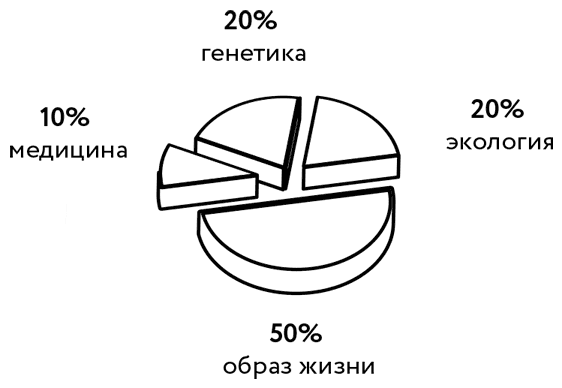
\includegraphics[width=0.5\textwidth]{willpower/pic4.png}
  %((карцінка: 10\% мэдыцына 20\% генэтыка 20\% экалёгія 50\% лад жыцьця))  
% \end{figure}

\paragraph{Рэсурсы здароўя мусяць адпавядаць асноўным крытэрам:} быць унівэрсальнымі для ўсіх людзей, мець надзейнае навуковае абгрунтаваньне свайго ўплыву на здароўе, быць даступнымі для самастойнай адзнакі і карэкцыі.

Усе рэсурсы шчыльна зьвязаныя паміж сабой, бо памяншэньне аднаго цягне за сабой памяншэньне шэрагу іншых. Слушная і зваротная залежнасьць: пры ўмацаваньні аднаго рэсурсу ўзмацняюцца і астатнія. Напрыклад, сон залежыць і ад фізычнай актыўнасьці, і ад рэжыму харчаваньня, і ад фактараў асяродзьдзя, і ад псыхалягічных фактараў.

% \begin{figure}[htb!]
%   \centering
%   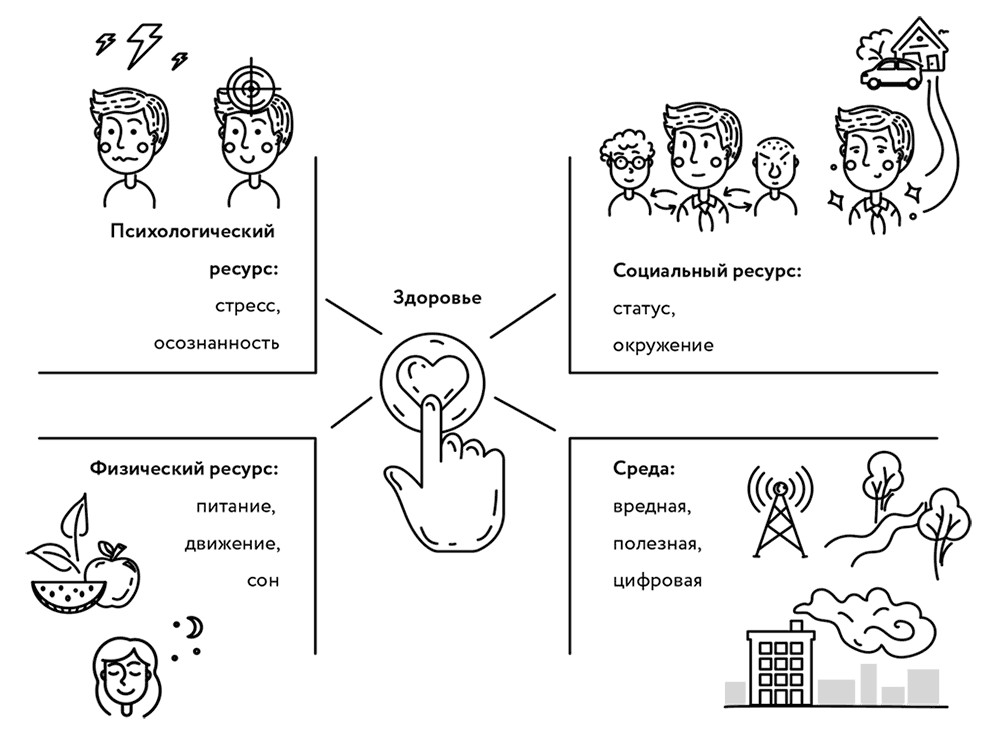
\includegraphics[width=1\textwidth]{willpower/pic5.png}
  % ((карцінка: Псыхалягічны рэсурс: стрэс, усьвядомленасьць Здароўе Сацыяльны рэсурс: статус, атачэньне Фізычны рэсурс: харчаваньне, рух, сон Асяродзьдзе: шкоднае, карыснае, лічбавае))
% \end{figure}

\paragraph{Базавымі зьяўляюцца фізычныя рэсурсы здароўя: рух, харчаваньне, сон і рэжым.} \textbf{Рух} уключае фізычную актыўнасьць любога віду (усе сытуацыі, калі вы не ляжыце, не сядзіце і не ясьце) і ўсіх разнавіднасьцяў (аэробныя, анаэробныя, зьмешаныя). А таксама цялеснасьць, гнуткасьць, цялесную адчувальнасьць, паставу і прафіляктыку траўмаў.
\textbf{Рэсурс харчаваньня} ўключае мноства навыкаў: гэта «што», «колькі», «калі» і «як» вы ясьце. Маюць значэньне ступень апрацоўкі, рэжым харчаваньня, стараннае жаваньне і нават кампанія за сталом.
\textbf{Сон і біярытмы}~--- ключавы рэсурс аднаўленьня: важна арганізаваць свой дзень у~аптымальны рэжым, узгадняючы рух, харчаваньне, стрэс, сьвятло, тэмпэратуру і шум. Важна сынхранізаваць усё, што мы робім, для лепшай аптымізацыі, і ўзгадніць з~натуральнай работай нашага ўнутранага гадзіньніка.

\paragraph{Псыхалягічныя рэсурсы ўключаюць стрэсаўстойлівасьць і ўсьвядомленасьць.} \textbf{Устойлівасьць} мяркуе ўменьне трываць высокі ўзровень стрэсу, выбіраць найбольш эфэктыўныя і дарэчныя копінг-стратэгіі (кагнітыўныя, эмацыйныя і паводніцкія спосабы справіцца са стрэсам), а~таксама ўнутраны локус кантролю і матывацыі. \textbf{Усьвядомленасьць} уключае ў~сябе ўменьне кіраваць сваёй увагай, быць спантанным, жыць у~моманце «тут і цяпер», з~разуменьнем і ўважлівасьцю ставіцца да эмоцыяў і перажываньняў сябе і іншых людзей, умець спачуваць, любіць, суперажываць.

\paragraph{Сацыяльныя рэсурсы здароўя ўключаюць сацыяльны статус і сацыяльнае асяродзьдзе і ўзаемадзеяньне.} \textbf{Сацыяльны статус} складаецца з~прыбытку, прывабнасьці, адукацыі і ўплыву. \textbf{Сацыяльнае асяродзьдзе}~--- гэта людзі, якія знаходзяцца вакол вас на рознай адлегласьці, але, як і статус, уплываюць на ваша здароўе. 

\emph{Гучыць страшна ці страшна цікава?}


\subsection*{Пытаньні і заданьні}

1. Якімі навыкамі і здаровымі звычкамі вы валодаеце, а~чаго вам бракуе?

2. Па якіх прыметах вы можаце вызначыць асабліва высокі ўзровень здароўя ў~сябе?

3. Як моцна працоўная нагрузка вычэрпвае вашыя рэсурсы здароўя? Ці надоўга вас стае?


\section{Залішняе здароўе}


Чаму многія старыя будынкі больш трывалыя за сучасныя? Калі архітэктар ня можа дакладна разьлічыць нагрузкі, ён імкнецца закласьці надмернасьць канструкцыі, робячы сьцены і перакрыцьці больш тоўстымі і надзейнымі. Такая надмернасьць і вядзе да даўгавечнасьці.

Калі я выкладаў у~мэдычным унівэрсітэце гісталёгію чалавека (навука аб будынку тканін і клетак, свайго роду «анатомія пад мікраскопам»), то часта дэманстраваў студэнтам існуючую «надмернасьць» практычна ўсіх органаў і тканак. Сапраўды, у~нас у~некалькі разоў больш, чым трэба, нэрвовых, цяглічных, злучальных клетак. Пры неабходнасьці чалавек можа жыць з~адным лёгкім, з~паловай кішачніка, печані, з~адной ныркай, нават з~дэфэктам прыкметнай часткі мозга. Прынцып надмернасьці зьвязаны як з~наяўнасьцю большай колькасьці элемэнтаў, чым трэба для функцыі, так і з~надмернасьцю каналаў перадачы інфармацыі, яе залішнім аб'ёмам.

Усе жывыя істоты, асобныя іх органы, тканкі і нават клеткі разьвіваюцца зь вялізным запасам надзейнасьці. Наша сьцегнавая костка вытрымлівае нагрузку ў~1,5 тоны, што амаль у~30 разоў перавышае звычайную нагрузку. Нашыя лёгкія здольныя пераносіць у~тры разы больш кіслароду, чым можа спатрэбіцца нават пры самых інтэнсіўных фізычных нагрузках.

\subsection*{Мо варта зэканоміць?} 

Цяпер прынята эканоміць на капітальных укладаньнях: чаму б не прыбраць адну нырку ці палову лёгкага, калі гэта не абмяжуе нас у~паўсядзённай жыцьцядзейнасьці? Аднак такая надмернасьць вельмі важная для выжываньня. Бо гэты запас дапамагае нам адаптавацца і перажыць цяжкую сытуацыю. 

\textbf{Чым большы «запас здароўя», тым большую нагрузку мы можам перанесьці, тым павольней будзем старэць пры згасаньні функцый. Чым вышэй мы падняліся, тым даўжэй будзем падаць.}

Таму так важна ведаць свой рэсурс. У нас можа ня быць прыкметаў хваробы, аднак калі рэсурсы здароўя зьніжаныя, то нават слабое ўзьдзеяньне можа выклікаць парушэньне функцый. Сапраўднае здароўе~--- гэта пацьверджаныя запасы здароўя. Калі людзі вядуць нездаровы лад жыцьця, то яны бяруць у~абавязак у~свайго здароўя, што павялічвае рызыку дрэннага самаадчуваньня. Перафразуючы філёзафа Фрыдрыха Ніцшэ: «Толькі лішак здароўя зьяўляецца доказам здароўя».

\subsection*{Надмернасьць і рызыка захворваньняў.} 

Мы ўжо казалі, што паніжаны рэсурс здароўя схіляе да захворваньня, а~высокі забясьпечвае добры ўзровень энэргічнасьці і прывабнасьці. 

Пры зьніжэньні рэсурсаў здароўя аслабляецца спантаннасьць, варыябэльнасьць рэгуляцыі асноўных сыстэм. Усё становіцца аднолькавым, стэрэатыпным, паўтаральным. Гэта датычыцца як зьніжэньня варыябэльнасьці сардэчнага рытму, так і зьбядненьня слоўнікавага запасу, скарачэньня даўжыні кроку і спантаннай фізычнай актыўнасьці, зьбядненьня рухальных патэрнаў, эмацыйнага выціску і шмат чаго іншага. Гэта прыкметы зьніжэньня здароўя нават у~фармальна здаровага чалавека.

\paragraph{Рэсурсы не зьяўляюцца інэртнымі.} Мы можам мабілізаваць сваю залішнюю магуту ў~выглядзе высокай працаздольнасьці, эмацыйнай стабільнасьці, увагі, сілы і розуму. Таму высокія рэсурсы здароўя~--- гэта наша штодзённае самаадчуваньне і магчымасьці. Нам трэба не «нармальнае» здароўе, а~«залішняе». Людзі з~разьвітай цяглічнай масай ня толькі мацнейшыя, але й здаравейшыя, бо цягліцы паглынаюць лішак глюкозы і тлушчу ў~крыві і абараняюць ад сардэчна-сасудзістых захворваньняў, падаўжаючы маладосьць. У спартоўцаў рызыка разьвіцьця астэапарозу значна меншая, бо да моманту старэньня і вытанчэньня шчыльнасьці касьцей іх косткі маюць большую вагу.

\subsection*{Кагнітыўны рэзэрв.}

30 гадоў таму навукоўцы, вывучаючы мозг, зьвярнулі ўвагу, што ў~часткі людзей пасьля сьмерці выяўляецца прыкметнае назапашваньне бляшак ды іншыя азнакі хваробы Альцгаймэра, але пры жыцьці ў~гэтых пацыентаў не было прыкметаў хваробы. Чаму? Аказалася, іх мозг быў крыху большы па масе і меў больш нэўронаў і сінаптычных сувязяў, чым у~сярэднім ва ўзроставай групе. Такім чынам, большы мозг абараняў і кампэнсаваў ужо ўзьніклыя нэўрадэгенэратыўныя захворваньні. Навукоўцы назвалі гэтую зьяву «кагнітыўны рэзэрв».

Пры навучаньні, інтэлектуальных намаганьнях, вывучэньні новага, уключаючы асваеньне нязвыклых рухальных патэрнаў, адбываецца стымуляцыя нэўрапластычнасьці на ўсіх узроўнях: сінаптычная пластычнасьць, нэўронавае рэмадэляваньне, нэўрагенэз~--- так-так, новыя нэўроны зьяўляюцца і ў~дарослых людзей. Чым больш назапашваецца новых атожылкаў і сувязяў, тым вышэйшы рэзерв. Макраскапічна гэта праяўляецца ў~выглядзе павелічэньня зьвілістасьці кары галаўнога мозгу. 

\tipbox{Анекдоты пра зьвіліны праўдзівыя: сапраўды, ёсьць карэляцыя паміж колькасьцю і глыбінёй зьвілінаў, інтэлектам і кагнітыўнай гнуткасьцю. А злоўжываньне алькаголем і траўмы галавы сапраўды могуць «выпрастаць» зьвіліны.}

Як мы ведаем, мозг плястычны, і атрыманыя, скажам, пры вывучэньні мовы новыя нэўронныя сувязі могуць зь лёгкасьцю выкарыстоўвацца для іншых задач. Пры захворваньні яны могуць узяць на сябе функцыі пашкоджаных структур, кампэнсуючы хваробу.

\tipbox{%Галоўнае~--- сэрцам не старэць!савецкая/расійская оптыка. Падумаю, чым адпаведным нашым можна замяніць 
Чым больш вы навучаецеся, прыкладаеце сьвядомых намаганьняў, трэніруеце ўвагу, тым больш значна памяншаецца рызыка дэмэнцыі.}

\emph{Так, рашэньне задач на ўвагу на 29 працэнтаў зьніжае рызыку дэмэнцыі празь 10 гадоў. Ежа для мозгу~--- гэта і рух, і, напрыклад, навучаньне ігры на музычным інструмэнце. Даведзена, што ў~групе аднаяйкавых блізьнятаў рызыка дэмэнцыі меншая на 64\,\% у~таго зь іх, хто вучыўся ў~музычнай школе. Назіраньні паказваюць, што білінгвы~--- людзі, якія напэраменку гавораць на дзьвюх мовах, -- захворваюць на Альцгаймэра на 4,3 гады пазьней, а~сымптомы ў~іх выяўляюцца на 5,1 года пазьней, чым у~людзей, якія размаўляюць на адной мове. У цэлым павышэньне мазгавой актыўнасьці на 33\,\% зьніжае рызыку разьвіцьця хваробы Альцгаймэра~--- вось такі эфэкт ведаў. Важныя для мозгу і камунікацыя, высокі ўзровень сацыяльнай актыўнасьці. Карміце ваш мозг якаснай ежай і разьвівайце карысныя сацыяльныя кантакты!}

Мы можам параўнаць кагнітыўны рэзэрв зь яшчэ адным паліўным бакам, які дазволіць нашаму мозгу даўжэй працаваць. Або з~запасным камандным пунктам, які возьме на сябе кіраваньне пры ўзьніклай праблеме. Выснова простая: лішніх ведаў не бывае. І запас тут не адцягвае кішэню, а~абараняе мозг. Чым больш у~вас інтэлектуальнай нагрузкі на працягу ўсяго жыцьця, тым вышэйшая вашая абарона ад старэньня мозгу, нэўралагічнай траўмы і шэрагу хваробаў. Чым вышэйшы ўзровень кагнітыўнага рэзэрву, тым зь меншым кагнітыўным дэфіцытам вы будзеце пераносіць нават ужо ўзьніклую хваробу. \textbf{Менавіта дзеля гэтага нам варта «бегчы з~усіх ног, каб толькі застацца на тым жа месцы».} Падобныя рэзэрвы існуюць і для іншых сыстэмаў арганізму. Напрыклад, вага касьцей. Калі чалавек на працягу жыцьця актыўна займаецца спортам, то ў~яго разьвітыя косткі і пры ўзроставым зьніжэньні шчыльнасьці касьцяной масы рызыка астэапарозу ў~яго меншая, чым у~чалавека зь ніжэйшай масай костак.

\subsection*{Прычыны здароўя, а~не прычыны хваробаў.}

Большасьць навукоўцаў доўгі час цікавілі перадусім пытаньні хваробаў. Важна было выявіць прычыны іх узьнікненьня, спосабы лячэньня і прафіляктыкі. Але затым усё больш дасьледнікаў пачалі ставіць пытаньне па-іншаму: «Адкуль бярэцца здароўе?» Бо нават пры эпідэміі захворваюць ня ўсе. У сытуацыі стрэсу бывае так, што частка людзей пачынае хварэць, але некаторыя, наадварот, становяцца мацнейшымі. Пры старэньні ў~розных людзей назіраюцца розныя траекторыі зьмены функцый. 

«Проста пашанцавала» ці ім нешта дапамагае?

\subsection*{Пытаньні і заданьні}

1. У якіх сфэрах жыцьця вы дзейнічаеце нашмат лепей, чым ад вас патрабуецца? Чаму? Якія перавагі вам прыносіць гэтая надмернасьць? Паглядзіце на розныя сфэры свайго жыцьця і скажыце сабе шчыра, дзе ў~вас «сярэдне» і «ў норме», а~дзе справы ідуць сапраўды добра. Якія паляпшэньні былі б для вас самыя жаданыя?

2. На колькі гадоў вы выглядаеце? А колькі гадоў вы б далі самі сабе? Колькі гадоў даюць вам навакольныя? Супастаўце гэтыя лічбы.

3. Пазыкі ці рэзэрвы? Складзіце сьпіс вашых пазыкаў і запасаў. Чым больш у~вас любых рэзэрваў~--- фінансавых, навыкаў, ведаў, сяброў, здароўя, матывацыі,~--- тым лепш. Добра было б раз на год падрахоўваць свае асобасныя рэзэрвы.


\section{Культура здароўя}

Да мяне на курсы часта прыходзяць людзі з~жаданьнем ня толькі палепшыць сваё самаадчуваньне, але і стварыць культуру здароўя ў~сям'і, каб паўплываць на сямейнікаў, каб дзеці вырасталі ў~асяродзьдзі, дзе культывуюцца і заахвочваюцца самаразьвіцьцё, здаровае харчаваньне, спорт. Калі мы ствараем такую атмасфэру, то яна падтрымлівае нас саміх і спрыяе засваеньню каштоўнасьцяў здароўя аўтаматычна. 

\tipbox{Калі вы вырасьлі ў~асяродзьдзі, дзе культуры здароўя не надавалася ўвагі, то ўсю працу трэба будзе прарабіць спачатку. Спадзяюся, гэтая кніга вам дапаможа.}

Здароўе~--- больш чым проста клопат пра сябе. Культура здароўя~--- гэта сацыяльная спадчыннасьць, гэта крышталізаваны вопыт і практыка, якія задаюць высокія стандарты ў~адносінах да сябе й іншых, вызначаюць каштоўнасьці і прыярытэты. Калі вы самі займаецеся здароўем, становіцеся прыкладам для сямейнікаў, сяброў, вы пераўтвараеце, аздараўляеце іх культурнае асяродзьдзе.

Дапамагаючы іншым людзям у~іх здароўі, падтрымліваючы і навучаючы, мы прапаведуем культуру здароўя. Добрыя ідэі не захопяць сьвет самі па сабе, патрэбныя асабісты прыклад і падтрымка. Стварайце свае групы ўплыву, навучайце~--- гэта выдатны спосаб і самаму глыбей пра нешта даведацца. Вядома, ня варта «задаваць дабро», навязваючы нешта іншым людзям, але дапамагаць тым, хто зьвернецца да вас з~пытаньнем,~--- важна і трэба.

\emph{У мяне падрастаюць трое сыноў, і я часта думаю аб тым, чаму я магу іх навучыць, што я магу ім даць. Як і любому з~бацькоў, мне хочацца, каб яны вырасьлі здаровым, разумнымі і актыўнымі. Навучаючы культуры здароўя сваіх дзяцей, мы даём ім у~спадчыну ня толькі гены, але й мэмы~--- здаровыя звычкі, якія спрыяюць росквіту.}

% ((карцінка: Культура здароўя: -Генэтычная спадчына (гены) -Эпігенэтычная спадчына -Культурная спадчына (мэмы) -Навучаньне здароўю))

Асновы здароўя закладваюцца ў~раньнія пэрыяды жыцьця, калі дзіця несьвядома капіюе паводзіны значных дарослых, перадусім бацькоў. Галоўнымі тут становяцца ня словы з~кніг, а~вашыя рэальныя дзеяньні, ваш уласны лад жыцьця. Навучаньне здароўю~--- гэта інвэстыцыя ў~культуру вашай сям'і, якая як каштоўнасьць можа перадавацца наступным пакаленьням.

Зьмяняючы сябе, мы ўплываем на наша асяродзьдзе. Мы хочам больш здаровых людзей, гарадоў, больш здаровай эканомікі і палітыкі. Культура здароўя~--- гэта рух ад здаровага харчаваньня да ўсьвядомленасьці, да спагады і ўзаемадапамогі. Гэта натуральная воля да жыцьця, інстынкт выжываньня, які змагаецца з~разбуральнымі тэндэнцыямі, накіраванымі на зьніжэньне чалавечай каштоўнасьці і годнасьці, на агрэсіўны маркетынг харчаваньня, баўленьня часу, небясьпечных для здароўя захапленьняў.

\emph{Я дзівуюся, што ёсьць партыі «Зялёных», але дасюль няма партыі «Здароўя». Бо «калі няма здароўя~--- маўчыць мудрасьць, ня можа расквітнець мастацтва, не гуляюць сілы, бескарыснае багацьце і хворы розум»Ведаць бы арыгінал~--- мо ёсьць на беларускую пераклад «сапраўдны», як пісалі яшчэ старажытныя грэкі.}

\subsection*{Мяккае ўспадкоўваньне.}

Тэрмінам «мяккае ўспадкоўваньне» часам пазначаюць зьмены актыўнасьці генаў, выкліканыя эпігенэтычнымі зьменамі (эпімутацыямі), як супрацьлегласьць «цьвёрдаму» ўспадкоўваньню, закадаванаму ў~пасьлядоўнасьці нуклеатыдаў ДНК. Пры гэтым могуць аднолькава перадавацца як нэгатыўныя, так і пазытыўныя прыкметы. Цікава, што пры захаваньні пастаянных вонкавых умоваў мяккае ўспадкоўваньне можа назапашвацца, і прыкметы будуць рабіцца больш выяўленымі. Суму эпігенэтычных мадыфікацый умоўна можна назваць эпігеномам. Асаблівасьць эпімутацый у~тым, што яны ўзьнікаюць пад узьдзеяньнем асяродзьдзя. Ёсьць меркаваньне, што сапраўдным інтэлігентам можа лічыцца толькі той, чые бабулі й дзядулі былі інтэлігентамі, і ніяк інакш.

\emph{Ёсьць вядомае дасьледаваньне пра стрэс і клопат у~пацукоў. Частыя кантакты з~маці ў~дзяцінстве прыводзяць да эпігенэтычнага мэтыляваньня праматораў генаў, якія адказваюць за стрэсавую рэакцыю. Таму ў~стрэсавых маці народзяцца больш стрэсавыя дзеці, якія будуць яшчэ горш клапаціцца пра сваіх нашчадкаў. Калі ж пацук-маці вельмі клапатлівая, то яе нашчадкі будуць такімі ж клапатлівымі.}

\emph{Калі з~боку маці ўспадкоўваюцца фактары цяжарнасьці і раньняга дзяцінства, то з~боку бацькаў сытуацыя складанейшая: уклад эпігенэтычнага ўспадкоўваньні з~іх боку нават мацнейшы праз інтэнсіўнае размнажэньне полавых клетак. Навукова даведзена, што нават без кантакту з~патомствам ад бацькаў можа перадавацца страх да некаторых пахаў. У экспэрымэнце навукоўцы выпрацавалі рэфлекс страху ў~мышэй на пах вішні, і высьветлілася, што страх перадаваўся на тры пакаленьні наперад~--- адчувальнымі да гэтага паху заставаліся і дзеці, і ўнукі «напалоханых» самцоў.}

Было даведзена, што схільнасьць да какаінавай залежнасьці таксама перадаецца праз бацькаў. Таму залежнасьці такія страшныя: яны ня толькі невылечныя пры жыцьці, але яшчэ і «дастаюцца ў~спадчыну» нашчадкам! Дасьледаваньні на жывёлах паказалі, што мышы, чые маці пераядалі, ужо зь дзяцінства аддаюць перавагу больш тлустай ежы. А вось рэгулярная фізычная актыўнасьць бацькоў здольная абараніць іх дзяцей ад мэтабалічных парушэньняў.

Істотна ўплывае на наша здароўе разьвіцьцё ў~вутробны пэрыяд. Моцны стрэс маці, узровень яе гармонаў, утрыманьне мінэралаў і вітамінаў~--- усё гэта аказвае доўгатэрміновае ўзьдзеяньне на здароўе і разьвіцьцё дзіцяці, закладвае яго траекторыю разьвіцьця на ўсё жыцьцё. Напрыклад, калі маці дрэнна харчавалася і дзіця нарадзілася з~вагой меншай за 2,5 кг, то ў~яго павышаная рызыка мэтабалічнага сындрому, цукровага дыябэту, сардэчна-сасудзістых захворваньняў. А калі дзіця нарадзілася з~вагой большай за 4,5 кг, то вышэйшая рызыка атлусьценьня, рака мозгу, тоўстага кішачніка, грудзей, падкарэньніцы (падкарэннай залозы).

Як можна выкарыстоўваць гэтыя веды? Вядома, не для скаргаў і абвінавачаньняў, маўляў, «продкі вінаватыя», а~для разуменьня таго, што, умацоўваючы сваё здароўе, даходы і культурны ўзровень, вы робіце гэта дзеля будучых пакаленьняў. Гэта рэальны эпігенэтычны дар, які будзе актуальны праз шмат гадоў, нават пасьля вашае сьмерці.

Узровень унутрывутробнага тэстастэрону і ў~мужчынаў, і ў~жанчынаў таксама мае вялікі ўплыў на разьвіцьцё мозгу і на рызыку шматлікіх захворваньняў, у~тым ліку і аўтызм, на асаблівасьці паводзінаў. На ўзровень тэстастэрону ў~маці ўплываюць яе атлусьценьне, цукровы дыябэт, хранічнае запаленьне і шэраг іншых прычын. 

\tipbox{Цяпер менавіта вы знаходзіцеся ў~пераломным пункце пераходу пакаленьняў зь мінулага ў~сучаснасьць, і менавіта ад вас залежыць, што перадасца: хваробы, залежнасьці і страхі або моцнае здароўе, клопат, стрэсаўстойлівасьць і высокі ўзровень жыцьця. Паляпшаючы сваё здароўе, вы паляпшае і здароўе вашых нашчадкаў!}

\subsection*{Выхаваньне здароўя.}

«Ня трэба іншага ўзору, калі перад вачыма прыклад бацькі». Акрамя геному, эпігенома, мікрабіёмы мы ўспадкоўваем ад бацькоў і «псыхом»~--- сукупнасьць мадэляў паводзінаў, установак і каштоўнасьцяў, прычым робім гэта некрытычна. Многія бацькі лічаць, што апранутае і накормленае дзіця~--- дастаткова для выхаваньня. А навучыць дзіця есьці, спаць, рухацца, даваць рады зь цяжкасьцямі, дапамагчы яму выставіць прыярытэты~--- гэта задача школы або настаўнікаў. Паверце, кінутае на самавыхаваньне дзіця засвоіць найгоршыя мадэлі паводзінаў. Калі вы не навучыце дзіця самі, іншыя навучаць яго быць зручным, падпарадкоўвацца і трываць.

Галоўны прынцып выхаваньня здароўя~--- пачаць зь сябе. Калі бацькі шчырыя зь дзецьмі, падтрымліваюць высокія асабістыя стандарты паводзінаў і маралі, дзеці засвойваюць гэта аўтаматычна. Бо, што б вы ні рабілі, вашыя дзеці ўсё роўна будуць падобныя да вас. Мы вучымся з~дапамогай люстраных нэўронаў, пераймаючы і капіюючы. Таму важна, каб у~жыцьці дзіцяці былі дарослыя з~жаданымі мадэлямі паводзінаў, і ня толькі бацькі. Калі вы не прытрымліваецеся тых каштоўнасьцяў, якія хочаце прывіць дзіцяці, ня трэба яго ашукваць і навязваць яму. Куды як лепей знайсьці іншага аўтарытэта, які прытрымліваецца гэтых правілаў, напрыклад добрага трэнэра.

Калі вы не выхоўваеце дзіця самі, то не дзівуйцеся потым, чаму яно паводзіцца інакш. Засвоіўшы пэўныя мадэлі паводзінаў у~дзяцінстве ў~дачыненьні да сну, харчаваньня, руху, усьвядомленасьці, чалавек кіруецца імі і ў~дарослым жыцьці. Дасьледаваньні паказваюць, што, калі здаровыя звычкі ўкараняюцца зь дзяцінства, іх узьдзеяньне максімальнае. Бо менавіта ў~пэрыяд росту і разьвіцьця закладваецца будучая траекторыя жыцьця дзіцяці.

\emph{Вывучайце зь дзіцем сваю сямейную гісторыю: важна, каб яно ганарылася сваім паходжаньнем, але пры гэтым ведала важнасьць і ўласных намаганьняў і магло дэманстраваць самадысцыпліну. Бо кантроль над сваімі імпульсамі~--- вагомы кампанэнт посьпеху. Чакайце ад дзіцяці посьпеху, кідайце яму выклікі і забясьпечвайце надзейную падтрымку, пазьбягаючы шкодных гіпэрапекі, жорсткасьці, эмацыйнай адстароненасьці.}

\subsection*{Чысты час для дзіцяці.}

Балюча глядзець на бацькоў, якія бавяць час зь дзецьмі, уткнуўшыся ў~смартфон. Чысты якасны час~--- гэта калі вы можаце надаць усю сваю ўвагу дзіцяці сам-насам, каб яму не давялося выпрошваць гэтыя хвіліны. Нават 15 хвілінаў такога чыстага часу могуць усё памяняць.

\emph{Як паказвае маштабнае дасьледаваньне, найважнейшым чыньнікам разьвіцьця мозгу дзіцяці і наступнай пасьпяховасьці зьяўляецца моўнае асяродзьдзе, у~якой яно знаходзіцца. Рацыянальным людзям, як я, цяжка зразумець, чаму зь немаўлятамі трэба і важна актыўна размаўляць, хоць яны й ня могуць нічога зразумець і пагатоў адказаць. Тамаграфія мозгу немаўлятаў паказвае, што яны актыўна апрацоўваюць маўленьне і нават у~думках прайграюць адказы на зьвернутыя да іх словы, нават калі яшчэ ня ўмеюць гаварыць. Так, сюсюканьне і насьпеў гукаў дапамагаюць дзіцяці лягчэй засвойваць веды. Колькасьць словаў, якія чуе дзіця, вызначае траекторыю яго навучаньня, матэматычныя навыкі і шматлікае іншае. Дзеці зь бедных сем'яў да трох гадоў чуюць на 30 мільёнаў словаў менш, чым дзеці з~заможных сем'яў, што прыкметна адбіваецца на іх далейшым лёсе.}

Важная накіраваная ўвага бацькоў, цяпло і бясьпека камунікацыі, патрэбныя ня толькі размовы па справе, але й «лішнія размовы». Ня толькі «еж, абуйся», але й «якая цікавая птушка сядзіць на клёне!». Чым больш працяглы дыялог, тым лепей для дзіцяці. Гаварыце пра тое, як вы верыце ў~яго,~--- чаканьні моцна ўплываюць. Гаварыце зь дзіцем пра яго бліжэйшае і далёкае мінулае і будучыню, такія размовы дапамагаюць яму прымаць лепшыя рашэньні ў~жыцьці. Бацькам важна займацца і сваёй самарэалізацыяй: чытайце больш кніг~--- гэта зробіць вашых дзяцей такімі ж, як вы. Давайце дзецям больш увагі ня толькі калі яны ідуць у~школу, але і ў~першыя гады жыцьця. 

Графік «крывая Хекмана» выразна дэманструе аддачу ад укладзеных у~чалавечы капітал сродкаў на розных этапах разьвіцьця: інвэстыцыі ў~раньняе дзяцінства нашмат больш эфэктыўныя, чым усе праграмы для пазьнейшага ўзросту.

\subsection*{Сон.}

З аднаго боку, важна падтрымліваць рэжым сну, усталёўваць выразныя межы і рытуалы. Але залішняя жорсткасьць шэрагу мэтадаў, калі дзіця пакідаюць плакаць на самоце і чакаюць, пакуль яно ня зьмірыцца з~адзінотай, небясьпечная і шкодная. Дзеці, якія сьпяць з~бацькамі, больш шчасьлівыя і менш палахлівыя ў~дарослым жыцьці. Самастойнасьць важная для дзіцяці тады, калі яно да яе гатовае.

Тыя падлеткі, якія сьпяць менш за 6 гадзінаў на содні, больш імпульсіўныя, схільныя да гвалту, суіцыду, часьцей ідуць на рызыкоўныя ўчынкі, часьцей ужываюць алькаголь і наркотыкі ў~параўнаньні з~тымі, хто сьпіць нармальна. Некаторыя бацькі выкарыстоўваюць сон як інструмэнт: напрыклад, заахвочваюць і ўзнагароджваюць дзяцей, дазваляючы ім ня класьціся позна ўвечары, караюць тым, што прымушаюць ісьці спаць раней. Гэта можа прывесьці да парушэньняў сну ў~будучыні.

\subsection*{Харчаваньне.}

Зь ежай падобная сытуацыя: многія бацькі выкарыстоўваюць ежу як соску, затыкаючы дзіця, калі яно плача. Ежай узнагароджваюць, многіх дзяцей прымусова закормліваюць, верагодна, лічачы, што чым больш зьела дзіця, тым больш яны клапатлівыя бацькі. У будучыні гэта можа прывесьці да парушэньняў харчовых паводзінаў. Не прымушайце дзяцей есьці і давайце ім права выбару ў~акрэсьленых вамі межах. Дзіўна, але многія бацькі то патураюць, то скардзяцца, што нічога ня могуць зрабіць. Правілы харчаваньня лёгка і проста замацоўваюцца, як і любая іншая звычка. Бацькі не павінныя перакладаць адказнасьць за харчаваньне на саміх дзяцей, апраўдваючы сябе тым, што «ён гэтага ня есьць», «яна гэтага ня хоча».

\subsection*{Рух.}

Абмежаваньне руху дзяцей і расстаньне зь імі пачынаецца ўжо ў~радзільнях, вядомых сваім жорсткім і агрэсіўным стаўленьнем да маці і тугім спавіваньнем дзяцей. Затым дзіця абмяжоўваюць у~руху, лаюць за тое, што яно лазіць, пэцкаецца, бегае, скача, шуміць. Але ж дзіця, якое не сваволіць,~--- імаверна, хворае дзіця! Рух для дзяцей~--- гэта ня толькі разьвіцьцё цела, але й разьвіцьцё мозгу, нават існуе такое паняцьце, як фізычны інтэлект.

\tipbox{Кожныя дзесяць гадоў трывушчасьць падлеткаў падае на 10\,\%, і 80\,\% зь іх не выконваюць мінімум рухальнай актыўнасьці. Кожныя дадатковыя 15 хвілінаў актыўнасьці ў~дзень павялічваюць на бал адзнакі дзяцей. Дзецям з~дэфіцытам увагі дастаткова толькі 20 хвілінаў фізкультуры, каб палепшыць упраўнасьць.}

Не ўлазьце ў~гульні і актыўнасьць дзяцей, давайце ім магчымасьць гуляць самастойна. Выключэньне~--- сытуацыі, дзе ўзьнікае рэальная (падкрэсьлю: рэальная) пагроза бясьпецы. Заахвочвайце актыўнасьць дзяцей з~самага раньняга ўзросту, прапануйце ім розныя віды актыўнасьці, але не настойвайце, калі яны ня хочуць. 

\tipbox{Не рабіце заўваг і папрокаў дзецям у~тым, што яны выпацкаліся, калі бегалі. Найлепшы спорт для дзяцей~--- гэта гульня. Гульні вучаць дзяцей узаемадзейнічаць, дамаўляцца паміж сабой.}

Чым больш рухаюцца бацькі, тым больш актыўныя і дзеці. На кожную дадатковую тысячу крокаў маці і таты дзеці праходзяць 200 дадатковых крокаў. Бацькі могуць навучыць дзіця атрымліваць задавальненьне ад руху, разьвіць у~ім уменьне трымаць паставу, уменьне валодаць сваім целам. 

\emph{Часам даць дзецям магчымасьць паварушыцца значыць вырашыць іх праблемы. Так, у~адным з~дасьледаваньняў магчымасьць рухацца падчас заняткаў зьнізіла гіпэрактыўнасьць і павысіла канцэнтрацыю і ўпраўнасьць дзяцей. Невыпадкова разьвіцьцю паставы заўсёды надавалася першараднае значэньне. Як выдатна сказаў Юрый Лотман: «Здольнасьць спатыкнуцца зьвязваецца не з~вонкавымі ўмовамі, а~з характарам і выхаваньнем чалавека. Душэўная і фізычная выкшталцонасьць зьвязаныя і выключаюць магчымасьць недакладных ці непрыгожых рухаў і жэстаў».}

У Крамянёвай даліне бацькі~--- топ-мэнэджары і заснавальнікі папулярных стартапаў~--- адкрываюць для сваіх дзяцей школы бяз гаджэтаў. Некантраляванае іх выкарыстаньне дзецьмі вядзе да таго, што яны менш сьпяць, у~іх вышэйшая рызыка дэпрэсіі, дыябэту, атлусьценьня, ніжэйшая шчыльнасьць костак.

Цяпер усё больш інфантыльных людзей. Важным у~выхаваньні зьяўляецца разьвіцьцё аўтаноміі і самастойнасьці дзіцяці. Многія мільярдэры аддаюць большую частку багацьця на дабрачыннасьць, пакідаючы дзецям толькі невялікую частку, каб яны не сталі закладнікамі грошай. Сталеньне~--- гэтае разьвіцьцё сваёй самастойнасьці, калі дзіця ясна разумее, што яму ніхто нічога не павінны і трэба вучыцца забясьпечваць сябе самастойна, а~не канькаць нешта ў~іншых людзей або чакаць ад дзяржавы.

Бацькам важна разьвіць незалежнасьць дзіцяці і навучыць яго паважаць межы іншых людзей, быць ветлівым і далікатным, не прэтэндаваць на чужое. Бо тое, што сапраўды належыць вам, у~вас немагчыма забраць!

\subsection*{Пытаньні і заданьні}

1. Якія здаровыя і нездаровыя звычкі вы скапіявалі ў~свайго асяродзядзя? Што ўзялі ад бацькоў?

2. Ці хацелі б вы разьвіць культуру здароўя ў~сваёй сям'і? Ці спрабавалі вы гэта зрабіць?

3. Якія са сваіх звычак вы хацелі б перадаць сваім дзецям? А якія~--- не? Складзіце сьпіс.

